% Options for packages loaded elsewhere
\PassOptionsToPackage{unicode}{hyperref}
\PassOptionsToPackage{hyphens}{url}
\PassOptionsToPackage{dvipsnames,svgnames,x11names}{xcolor}
%
\documentclass[
  11pt,
  letterpaper,
  DIV=11,
  numbers=noendperiod]{scrartcl}

\usepackage{amsmath,amssymb}
\usepackage{setspace}
\usepackage{iftex}
\ifPDFTeX
  \usepackage[T1]{fontenc}
  \usepackage[utf8]{inputenc}
  \usepackage{textcomp} % provide euro and other symbols
\else % if luatex or xetex
  \usepackage{unicode-math}
  \defaultfontfeatures{Scale=MatchLowercase}
  \defaultfontfeatures[\rmfamily]{Ligatures=TeX,Scale=1}
\fi
\usepackage{lmodern}
\ifPDFTeX\else  
    % xetex/luatex font selection
\fi
% Use upquote if available, for straight quotes in verbatim environments
\IfFileExists{upquote.sty}{\usepackage{upquote}}{}
\IfFileExists{microtype.sty}{% use microtype if available
  \usepackage[]{microtype}
  \UseMicrotypeSet[protrusion]{basicmath} % disable protrusion for tt fonts
}{}
\makeatletter
\@ifundefined{KOMAClassName}{% if non-KOMA class
  \IfFileExists{parskip.sty}{%
    \usepackage{parskip}
  }{% else
    \setlength{\parindent}{0pt}
    \setlength{\parskip}{6pt plus 2pt minus 1pt}}
}{% if KOMA class
  \KOMAoptions{parskip=half}}
\makeatother
\usepackage{xcolor}
\setlength{\emergencystretch}{3em} % prevent overfull lines
\setcounter{secnumdepth}{-\maxdimen} % remove section numbering
% Make \paragraph and \subparagraph free-standing
\ifx\paragraph\undefined\else
  \let\oldparagraph\paragraph
  \renewcommand{\paragraph}[1]{\oldparagraph{#1}\mbox{}}
\fi
\ifx\subparagraph\undefined\else
  \let\oldsubparagraph\subparagraph
  \renewcommand{\subparagraph}[1]{\oldsubparagraph{#1}\mbox{}}
\fi


\providecommand{\tightlist}{%
  \setlength{\itemsep}{0pt}\setlength{\parskip}{0pt}}\usepackage{longtable,booktabs,array}
\usepackage{calc} % for calculating minipage widths
% Correct order of tables after \paragraph or \subparagraph
\usepackage{etoolbox}
\makeatletter
\patchcmd\longtable{\par}{\if@noskipsec\mbox{}\fi\par}{}{}
\makeatother
% Allow footnotes in longtable head/foot
\IfFileExists{footnotehyper.sty}{\usepackage{footnotehyper}}{\usepackage{footnote}}
\makesavenoteenv{longtable}
\usepackage{graphicx}
\makeatletter
\def\maxwidth{\ifdim\Gin@nat@width>\linewidth\linewidth\else\Gin@nat@width\fi}
\def\maxheight{\ifdim\Gin@nat@height>\textheight\textheight\else\Gin@nat@height\fi}
\makeatother
% Scale images if necessary, so that they will not overflow the page
% margins by default, and it is still possible to overwrite the defaults
% using explicit options in \includegraphics[width, height, ...]{}
\setkeys{Gin}{width=\maxwidth,height=\maxheight,keepaspectratio}
% Set default figure placement to htbp
\makeatletter
\def\fps@figure{htbp}
\makeatother
% definitions for citeproc citations
\NewDocumentCommand\citeproctext{}{}
\NewDocumentCommand\citeproc{mm}{%
  \begingroup\def\citeproctext{#2}\cite{#1}\endgroup}
\makeatletter
 % allow citations to break across lines
 \let\@cite@ofmt\@firstofone
 % avoid brackets around text for \cite:
 \def\@biblabel#1{}
 \def\@cite#1#2{{#1\if@tempswa , #2\fi}}
\makeatother
\newlength{\cslhangindent}
\setlength{\cslhangindent}{1.5em}
\newlength{\csllabelwidth}
\setlength{\csllabelwidth}{3em}
\newenvironment{CSLReferences}[2] % #1 hanging-indent, #2 entry-spacing
 {\begin{list}{}{%
  \setlength{\itemindent}{0pt}
  \setlength{\leftmargin}{0pt}
  \setlength{\parsep}{0pt}
  % turn on hanging indent if param 1 is 1
  \ifodd #1
   \setlength{\leftmargin}{\cslhangindent}
   \setlength{\itemindent}{-1\cslhangindent}
  \fi
  % set entry spacing
  \setlength{\itemsep}{#2\baselineskip}}}
 {\end{list}}
\usepackage{calc}
\newcommand{\CSLBlock}[1]{\hfill\break\parbox[t]{\linewidth}{\strut\ignorespaces#1\strut}}
\newcommand{\CSLLeftMargin}[1]{\parbox[t]{\csllabelwidth}{\strut#1\strut}}
\newcommand{\CSLRightInline}[1]{\parbox[t]{\linewidth - \csllabelwidth}{\strut#1\strut}}
\newcommand{\CSLIndent}[1]{\hspace{\cslhangindent}#1}

\usepackage{booktabs}
\usepackage{longtable}
\usepackage{array}
\usepackage{multirow}
\usepackage{wrapfig}
\usepackage{float}
\usepackage{colortbl}
\usepackage{pdflscape}
\usepackage{tabu}
\usepackage{threeparttable}
\usepackage{threeparttablex}
\usepackage[normalem]{ulem}
\usepackage{makecell}
\usepackage{xcolor}
\KOMAoption{captions}{tableheading}
\usepackage{textcomp}
\usepackage{utopia}
\usepackage{lineno}
\usepackage[utf8]{inputenc}
\linenumbers
\usepackage{float}
\floatplacement{figure}{H}
\usepackage{caption}
\captionsetup[figure]{font=scriptsize}
\captionsetup[table]{font=scriptsize}

\makeatletter
\@ifpackageloaded{caption}{}{\usepackage{caption}}
\AtBeginDocument{%
\ifdefined\contentsname
  \renewcommand*\contentsname{Table of contents}
\else
  \newcommand\contentsname{Table of contents}
\fi
\ifdefined\listfigurename
  \renewcommand*\listfigurename{List of Figures}
\else
  \newcommand\listfigurename{List of Figures}
\fi
\ifdefined\listtablename
  \renewcommand*\listtablename{List of Tables}
\else
  \newcommand\listtablename{List of Tables}
\fi
\ifdefined\figurename
  \renewcommand*\figurename{Figure}
\else
  \newcommand\figurename{Figure}
\fi
\ifdefined\tablename
  \renewcommand*\tablename{Table}
\else
  \newcommand\tablename{Table}
\fi
}
\@ifpackageloaded{float}{}{\usepackage{float}}
\floatstyle{ruled}
\@ifundefined{c@chapter}{\newfloat{codelisting}{h}{lop}}{\newfloat{codelisting}{h}{lop}[chapter]}
\floatname{codelisting}{Listing}
\newcommand*\listoflistings{\listof{codelisting}{List of Listings}}
\makeatother
\makeatletter
\makeatother
\makeatletter
\@ifpackageloaded{caption}{}{\usepackage{caption}}
\@ifpackageloaded{subcaption}{}{\usepackage{subcaption}}
\makeatother
\ifLuaTeX
  \usepackage{selnolig}  % disable illegal ligatures
\fi
\usepackage{bookmark}

\IfFileExists{xurl.sty}{\usepackage{xurl}}{} % add URL line breaks if available
\urlstyle{same} % disable monospaced font for URLs
\hypersetup{
  pdftitle={Variation matters: Expanding the scope of experimental archaeology using the Perception-Process-Product conceptual framework},
  pdfauthor={Cheng Liu},
  colorlinks=true,
  linkcolor={blue},
  filecolor={Maroon},
  citecolor={Blue},
  urlcolor={Blue},
  pdfcreator={LaTeX via pandoc}}

\title{Variation matters: Expanding the scope of experimental
archaeology using the Perception-Process-Product conceptual framework}
\author{Cheng Liu\footnote{Department of Anthropology, Emory University,
  Atlanta, GA, USA; cheng.liu@emory.edu}}
\date{2024-05-12}

\begin{document}
\maketitle
\begin{abstract}
This paper presents the Perception-Process-Product (``Triple P'')
framework that aims to expand the scope of experimental archaeology. The
Triple P framework emphasizes multi-level variation and interactions
across the levels of perception, process, and product to provide a more
grounded and richer explanation of the past archaeological record. It
consists of three principles: 1) acknowledging the inherent trade-off
between control and generalizability in the experimental research
design; 2) encouraging collaborative projects that involve
geographically diverse and non-traditional research participants such as
hobbyists and novices; 3) adopting a workflow that normalizes the
collection and curation of ethological and ethnographic data in
experimental projects. Serving as a heuristic device, this alternative
mode of knowledge production is highly flexible in nature, where each
single component is detachable as dicated by individual research
question.
\end{abstract}

\setstretch{1.5}
\keywords{Experimental archaeology; Ethological analysis; Ethnographic research; Curse of knowledge; Collaborative knowledge production}

\section{Introduction}\label{introduction}

This paper presents the Perception-Process-Product (hereafter ``Triple
P'') conceptual framework to expand the scope of experimental
archaeology. The field has long tended to adopt the principle of Occam's
razor (e.g., \citeproc{ref-blessing2021}{Blessing \& Schmidt, 2021};
\citeproc{ref-domuxednguez-rodrigo2008}{Domínguez-Rodrigo, 2008};
\citeproc{ref-reeves2009}{Reeves et al., 2009};
\citeproc{ref-schmidt2019}{P. Schmidt et al., 2019}), whether explicitly
or implicitly. This assumption acts to center inquiry around the reverse
engineering of a past technology in a minimal or least-effort manner
while ignoring the rich contextual information experimentation affords.
When applied to the experimental study of ancient craftsmanship, Occam's
razor, or the law of parsimony, implies that a technological solution
that is simpler to reproduce is more likely to be the one used in the
archaeological context. This is insufficient to infer the preferences of
``irrational'' agents possessing incomplete information
(\citeproc{ref-armstrong2018}{Mindermann \& Armstrong, 2018}) in tool
design and use. The two conditions described here provide a better
approximation of past humans displaying extensive cultural variation as
opposed to the assumption of omniscient \emph{Homo economicus} (i.e.,
the idea that humans are consistently rational and narrowly
self-interested agents pursuing optimality) that has been rejected by
many anthropologists (\citeproc{ref-apicella2020}{Apicella et al.,
2020}; \citeproc{ref-henrichSearchHomoEconomicus2001}{Henrich et al.,
2001}). Heyes (\citeproc{ref-heyes2012}{Heyes, 2012}) similarly
questioned the abuse of parsimony in animal behavioral research and
proposed that new observational and experimental studies that allow
differential predictions to be tested become necessary when both a
simple and a complex mechanism can explain the phenomenon of interest.

In fact, there are several reasons why past technologies may violate
``parsimonious'' assumptions of minimal manufacture complexity and
optimal functional efficiency. In the evolution of technology, it is
rather common that opaque causal perception and its resulting tendency
of over-imitation can lead to the widespread and long-lasting
reproduction of technological solutions that are neither minimal in
manufacture complexity nor optimal in functional efficiency.
Over-imitation means the copying of actions that are causally irrelevant
in a goal-directed action sequence (\citeproc{ref-lyons2007}{Lyons et
al., 2007}). It is a psychological propensity that was suggested to be
uniquely prevalent among humans when comparing with non-human primates
including chimpanzees (\citeproc{ref-horner2005}{Horner \& Whiten,
2005}), bonobos (\citeproc{ref-clay2018}{Clay \& Tennie, 2018}) and
orangutans (\citeproc{ref-nielsenFailureFindOverimitation2010}{Nielsen
\& Susianto, 2010}). Subsequent research further suggested that within
human societies over-imitation has been commonly observed among children
across various cultural contexts (\citeproc{ref-berl2015}{Berl \&
Hewlett, 2015}; \citeproc{ref-nielsen2014}{Nielsen et al., 2014};
\citeproc{ref-nielsen2010}{Nielsen \& Tomaselli, 2010};
\citeproc{ref-stengelin2020}{Stengelin et al., 2020};
\citeproc{ref-subiaul2016}{Subiaul et al., 2016}). Gergely and Csisbra
(\citeproc{ref-gergely2006}{2006}) introduced ``Sylvia's Recipe'' that
vividly illustrates this cognitive process in the transmission of
technical skills. Sylvia is an education researcher who developed a
unique way of cooking ham roast by observing her mother during
childhood, where she cut both ends of a ham. Later in life, her mother
happened to watch her cooking, where she noticed and questioned the
purpose of this step of preparation. Sylvia could not answer it and was
then told that it was processed that way because her mother did not have
a pan that was large enough to cook a full-sized ham. The commonality of
this opaque causal perception has also been demonstrated in a recent
study of Hadza bowmakers. Harris et al.
(\citeproc{ref-harris2021}{2021}) found that even experienced bowmakers
only possess limited causal knowledge regarding the design and
construction of bows according to modern engineering principles, meaning
they cannot spell out the mechanical (dis)advantages of many
morphological features.

On the other hand, path dependence also constrained the pursuit of
functional optimization or simplification of manufacturing procedures.
In this case, people are implicitly or explicitly aware of the existence
of a more efficient solution but still stick to the older one due to the
cost of learning, cultural conservatism
(\citeproc{ref-acerbi2009}{Acerbi et al., 2009};
\citeproc{ref-ghirlanda2006}{Ghirlanda et al., 2006};
\citeproc{ref-morin2022}{Morin, 2022}), or other reasons. One such
example in the evolution of technology is the longevity of QWERTY
keyboard design (\citeproc{ref-kafaee2022}{Kafaee et al., 2022}). This
deliberately unergonomic solution was invented in the era of typewriters
in order to disperse commonly used letters, preventing the most
frequently struck ``hammers'' from clashing. Yet it is still the most
common keyboard design today when such constraint does not exist anymore
on modern computer hardware. In short, we should acknowledge the
existence and variation of many ``good-enough'' technological solutions
featuring various degrees of ``redundancy'' in real-world contexts,
which often represent locally adaptive peaks instead of a global optimum
in a multimodal fitness landscape due to multiple constraints and
trade-off factors (\citeproc{ref-bettinger1982}{Bettinger \& Baumhoff,
1982}; \citeproc{ref-mesoudi2008}{Mesoudi \& O'Brien, 2008}).

Built upon this critique of \emph{Homo economicus} as well as the four
strategies\^{}{[}Strategy 2 is particularly relevant here, which is
``the pursuit of general questions in present-day material culture in
order to acquiring laws for making useful behavioral inferences''
(Schiffer, 2010: 6){]} of behavioral archaeology
(\citeproc{ref-reid1975}{Reid et al., 1975};
\citeproc{ref-schiffer2010}{Schiffer, 2010}), here I propose the Triple
P framework, which aims to \textbf{a)} amplify the expression of
variation in experimental replicas (product) and their associated
behavioral channels (process) as well as sensory experiences
(perception) by experiments in diverse contexts and \textbf{b)} better
identify the complex interacting relationships across these three levels
of variations in real-world conditions. To accomplish these two
objectives, I advocate the following three principles as integral
components of the Triple P framework, which requires \textbf{1)}
acknowledging the inherent trade-off between control and
generalizability in the experimental research design and \textbf{2)}
encouraging collaborative projects that involve geographically diverse
and non-traditional research participants such as hobbyists and novices.
These two principles are developed to advocate a pluralistic approach to
the explanation of complex variation, which has received more attention
from evolutionary anthropology (\citeproc{ref-antuxf3n2017}{Antón \&
Kuzawa, 2017}) to cognitive science (\citeproc{ref-barrett2020}{Barrett,
2020}), instead of treating the optimization-based research agenda as a
panacea. The second principle particularly allows researchers to develop
research questions that are also meaningful to descendant communities
through respectful conversation and collaboration
(\citeproc{ref-montgomery2023}{Montgomery \& Fryer, 2023}). The Triple P
framework also \textbf{3)} adopts a workflow that normalizes the
collection and curation of ethological and ethnographic data in
experimental projects. It is acknowledged that strategies of data
collection and analysis of a given experimental project should be
primarily derived from the research question, but the awareness of the
rich toolkit available can sometimes inspire researchers to ask
questions that are bold and transformative
(\citeproc{ref-schmidt2020}{S. C. Schmidt \& Marwick, 2020}). Here I
will leverage the extensive corpus in experimental designs and
inferences revolving around stone artifacts to clarify its meaning and
demonstrate the necessity and potential of this framework.

\section{What good is less-controlled
experimentation?}\label{what-good-is-less-controlled-experimentation}

The trade-off between causal inference (aka ``internal validity'') and
generalization (aka ``external validity'') forms a central issue in
experimental design across different disciplines
(\citeproc{ref-eren2016}{Eren et al., 2016}; \citeproc{ref-roe2009}{Roe
\& Just, 2009}: 1266-1267). Even in fields known for their development
of rigorous and well-controlled experimental methods such as cognitive
psychology and neuroscience, researchers have started to use relatively
naturalistic stimuli more frequently and advocate a paradigm shift to
semi-controlled experiments due to the generalizability crisis, namely
the prevailing mismatch between phenomenon of interest and measured
variables in psychological science (\citeproc{ref-nastase2020}{Nastase
et al., 2020}; \citeproc{ref-shamay-tsoory2019}{Shamay-Tsoory \&
Mendelsohn, 2019}; \citeproc{ref-sonkusare2019}{Sonkusare et al., 2019};
\citeproc{ref-yarkoni2022}{Yarkoni, 2022}). In contrast, the past
decades have witnessed experimental archaeology's growing research
interests focusing on the robust inference of causal mechanisms while
compromising generalizability in the explanation of material culture
variation (\citeproc{ref-eren2016}{Eren et al., 2016};
\citeproc{ref-eren2024}{Eren \& Meltzer, 2024};
\citeproc{ref-lin2018}{Lin et al., 2018};
\citeproc{ref-marreiros2020}{Marreiros et al., 2020}). In the context of
stone artifact replication, one typical research design emphasizing
causality over generalizability is the use of knapping machines/robots
(\citeproc{ref-li2022}{Li et al., 2022};
\citeproc{ref-pfleging2019}{Pfleging et al., 2019}), which has helped
map out the physical constraints of stone artifact manufacture and use
through the identification of causal relationships between input (force,
exterior platform angle, platform depth, etc.) and outcome variables
(flake size, flake shape, wear formation, etc.). All variables of
interest in this setting are relatively easy to measure, quantify, and
control, but this type of design can be insufficient in inferring how
context-generic principles interact in a particular context as reflected
in real-world conditions. This research orientation prioritizes the
material science aspect over the social science aspect of experimental
archaeology. Similarly, standardized artificial materials like bricks
(\citeproc{ref-lombao2017}{Lombao et al., 2017}) or foam blocks
(\citeproc{ref-schillinger2016}{Schillinger et al., 2016}) have been
used to standardize materials and/or reduce learning demands in
experimental studies focusing on the transmission of lithic
technologies, with implications for the generalizability of results
(\citeproc{ref-liu2023}{Liu et al., 2023}). In real-world knapping, each
rock has a different shape and often different physical properties such
as inner cracks and inclusions, and this heterogeneity itself represents
a critical variable in cultural transmission and skill development
(\citeproc{ref-proffitt2022}{Proffitt et al., 2022}).

On the other hand, less-controlled experiments, which have been
traditionally known as naturalistic or actualistic experiments (see
\citeproc{ref-conrad2023}{Conrad et al., 2023};
\citeproc{ref-eren2024}{Eren \& Meltzer, 2024} for detailed
terminological critiques), pay more attention to how experimental
insights can be generalized to archaeological samples by incorporating
authentic materials and plausible social settings with a certain degree
of compromised control (\citeproc{ref-outram2008}{Outram, 2008}). Back
to the cases of cultural transmission experiments, a less-controlled
experiment would involve the use of natural rocks with varied morphology
instead of standardized artificial materials as well as human
demonstrators instead of videos of knapping instruction, despite the
fact that the latter will remain consistent across individuals. Unlike
strictly controlled experiments testing one variable of interest each
time (\citeproc{ref-almaatouq2024}{Almaatouq et al., 2024}),
less-controlled experiments are designed to produce variation and their
interactions. This feature is crucial and cannot be simply replaced by
ethnographic records or ethnoarchaeology, because many paleolithic
technological components do not have analogs in contemporary
non-industrial societies (e.g., \citeproc{ref-arthur2018}{Arthur, 2018};
\citeproc{ref-stout2002}{Stout, 2002}). While uncontrolled variation has
traditionally been viewed as highly problematic, statistical techniques
for developing causal inference from observational data, of the kind
produced by less-controlled experiments, have also been greatly boosted
in epidemiology and economics in recent years
(\citeproc{ref-cunningham2021}{Cunningham, 2021};
\citeproc{ref-hernan2023}{Hernan \& Robins, 2023}). Despite the fact
that one should not interpret any experiment as a direct representation
of an actual past event (\citeproc{ref-eren2024}{Eren \& Meltzer,
2024}), less-controlled experiments can serve a heuristic role in
hypothesis generation, aligning with the perspective of Lin et al.
(\citeproc{ref-lin2018}{2018}: 680-681), who proposed that the
interaction between less-controlled and strictly controlled experiments
``operates in a cyclical form of induction and deduction.''

\section{Many places, many voices}\label{many-places-many-voices}

Traditional practices in experimental archaeology, as manifested by the
fact that a majority of scholarly publications are produced as results
of experiments conducted by a single knapper with the dual identity of
also being a researcher (\citeproc{ref-whittaker2004}{Whittaker, 2004}),
tend to be restrained by the cognitive bias known as the ``curse of
knowledge'' or ``curse of expertise.'' This psychological term
originally refers to the phenomenon that it is extremely challenging for
experts to ignore the information that is held by them but not others,
particularly novices, when communicating with others
(\citeproc{ref-hinds1999}{Hinds, 1999}), but it has further implications
for the sample representativeness in experimental archaeology. When the
knapping expertise is gradually formed through multiple years of
observations and trial-and-error learning, an expert knapper develops
some specific ways of strategic planning, motor habits (and their
associated impacts on anatomical forms like wrist and elbow),
preferences of percussor and raw material types, as well as familiarity
of various techniques that become unforgettable
(\citeproc{ref-moore2020}{Moore, 2020}: 654). The existence of this
cognitive bias is not inherently bad, and these many years of experience
should be appreciated and celebrated by experimental archaeologists.
However, what is problematic is that the results of replication
experiments conducted by these experienced practitioners, often in
settings of single knapper, have been constantly framed as
generalizations regarding the evolution of technology and cognition that
masks a vast range of technological diversity.

Modern flintknapping techniques, as a research subject and a scientific
method, originated from hobbyists' individualistic trials of reverse
engineering during the 19th century (\citeproc{ref-coles1979}{Coles,
1979}; \citeproc{ref-flenniken1984}{Flenniken, 1984};
\citeproc{ref-johnson1978}{Johnson, 1978};
\citeproc{ref-whittaker1994}{Whittaker, 1994}: 54-61). Hobbyist knappers
represent a huge repertoire of technological knowledge that does not
fully overlap with what is acquired by academic knappers. They tend to
generate ideas that may appear to be counter-intuitive at first glance
for academics. One such example is the utility of obtuse edge angle as
demonstrated by Don Crabtree (\citeproc{ref-crabtree1977}{1977}), a
mostly self-educated flintknapper yet one of the most important figures
in experimental archaeology. In his experiment, Crabtree demonstrated
the excellent performance of blade dorsal ridge on tasks like shaving
and cutting hard materials, challenging the traditional perspective on
producing sharp lateral edges as the sole purpose of stone toolmaking
and shedding light on future functional reconstruction through the
use-wear analysis. It is rather unfortunate that collaborations between
academics and hobbyists are less common than expected due to their
complicated and uneasy relationships as detailed in Whittaker's
(\citeproc{ref-whittaker2004}{2004}) ethnography. Likewise, novices'
lack of flintknapping expertise also helps to mitigate the ``curse of
knowledge'' bias that may hinder expert knappers. Their involvement can
potentially lead to the discovery of alternative methods, techniques,
and interpretations that may have been overlooked by experts. Several
researchers have also pointed out that the literature-informed
archaeologists sometimes get lost in reconstructing previous
archaeologists' reconstructions instead of searching for diverse
solutions to better understand the actual archaeological phenomenon
(\citeproc{ref-bell2014}{Bell, 2014}; \citeproc{ref-currie2022}{Currie,
2022}), which is another reason why we need the presence of hobbyists
and novices in the community of experimental archaeology.

Emphasizing variation at its core, the Triple P conceptual framework
recognizes that experimental archaeology can greatly benefit from
diverse perspectives (\citeproc{ref-pargeter2023}{Pargeter et al.,
2023}: 164) and thereby inherently adopts a collaborative mode of
knowledge production, which has been recently advocated in experimental
studies (\citeproc{ref-liuInferringCulturalReproduction2023}{Liu \&
Stout, 2023}; \citeproc{ref-ranhorn2020}{Ranhorn et al., 2020}) and
museum collection studies (\citeproc{ref-timbrell2023}{Timbrell, 2023})
of stone artifacts. Furthermore, the Triple P framework acknowledges
that communities living in specific geographical areas possess unique
insights and understanding of their cultural heritage
(\citeproc{ref-arthur2024}{Arthur et al., 2024}). This emphasis on team
efforts and inclusivity allows for a more complete understanding of the
non-utilitarian or unexpected aspects of raw material procurement
(\citeproc{ref-batalla2016}{Batalla, 2016}) and selection
(\citeproc{ref-arthur2021}{Arthur, 2021}), pre-treatment
(\citeproc{ref-maloney2020}{Maloney \& Street, 2020}), production
(\citeproc{ref-griffin2013}{Griffin et al., 2013}), and use
(\citeproc{ref-martellotta2022}{Martellotta et al., 2022};
\citeproc{ref-milks2023}{Milks et al., 2023}) across different regions.
Through ethical collaborations with those knapping practitioners in
non-industrial societies in the research process, the framework allows
their voices to be heard and their contributions to be acknowledged.
This not only enhances the quality of research outcomes but also fosters
a sense of ownership and pride within these communities, strengthening
the connection between archaeological research and the people it
directly affects (\citeproc{ref-douglass2020}{Douglass, 2020};
\citeproc{ref-marshall2002}{Marshall, 2002};
\citeproc{ref-montgomery2023}{Montgomery \& Fryer, 2023}).

However, the facilitation of large-scale collaborations faces challenges
within the current system of research evaluation. The prevailing
practice of attributing credit primarily to the first author and senior
(last/corresponding) author in peer-reviewed journal papers hampers the
recognition of multiple contributors. This system often overlooks the
valuable input of collaborators who may not fit into the traditional
authorship structure but have made significant intellectual and
practical contributions to the research. To truly embrace the principles
of collaboration and inclusivity, there is a need for a reevaluation of
the research evaluation system, allowing for proper acknowledgment of
the diverse voices and contributions involved in large-scale
collaborations (\citeproc{ref-ouzman2023}{Ouzman, 2023}). Moreover,
considering the broader social context of the checkered disciplinary
history of archaeology/anthropology featuring colonial exploitation, the
changes in the evaluation system alone are not enough. This further
highlights the need for adopting a community-based approach to
fundamentally transform the power dynamics in archaeological knowledge
production and distribution (\citeproc{ref-atalay2012}{Atalay, 2012};
\citeproc{ref-lasalle2010}{La Salle, 2010};
\citeproc{ref-schneider2020}{Schneider \& Hayes, 2020}).

\section{The Triple P framework in
action}\label{the-triple-p-framework-in-action}

The implementation of the Triple P framework involves the collection of
process-level (ethological) and perception-level (ethnographic) data
(\textbf{Figure} @ref(fig:concept)), which is critical to address
equifinality and multifinality
(\citeproc{ref-erenExperimentalBisonButchery2024}{Eren et al., 2024};
\citeproc{ref-hiscock2004}{Hiscock, 2004}; \citeproc{ref-nami2010}{Nami,
2010}; \citeproc{ref-premoEquifinalityExplanationThoughts2010}{Premo,
2010}), two daunting challenges in archaeological inference.
Equifinality refers to situations in which a similar state or
consequence can be achieved through multiple different paths, while
multifinality emerges when a similar process can lead to multiple ends.
While we cannot fully solve these two problems and accurately
reconstruct the past behavioral processes simply based on materials
remains, context-rich experiments involving the collection of
ethological and ethnographic data can help us better document an
enlarged range of possible combinations of variation and draw a more
informed inference (\citeproc{ref-reynolds1999}{Reynolds, 1999}). The
importance of specifying and documenting the context information of both
the experiment and the phenomenon of interest has also been recently
highlighted in psychological sciences
(\citeproc{ref-holleman2020}{Holleman et al., 2020}).

\begin{figure}[H]

{\centering 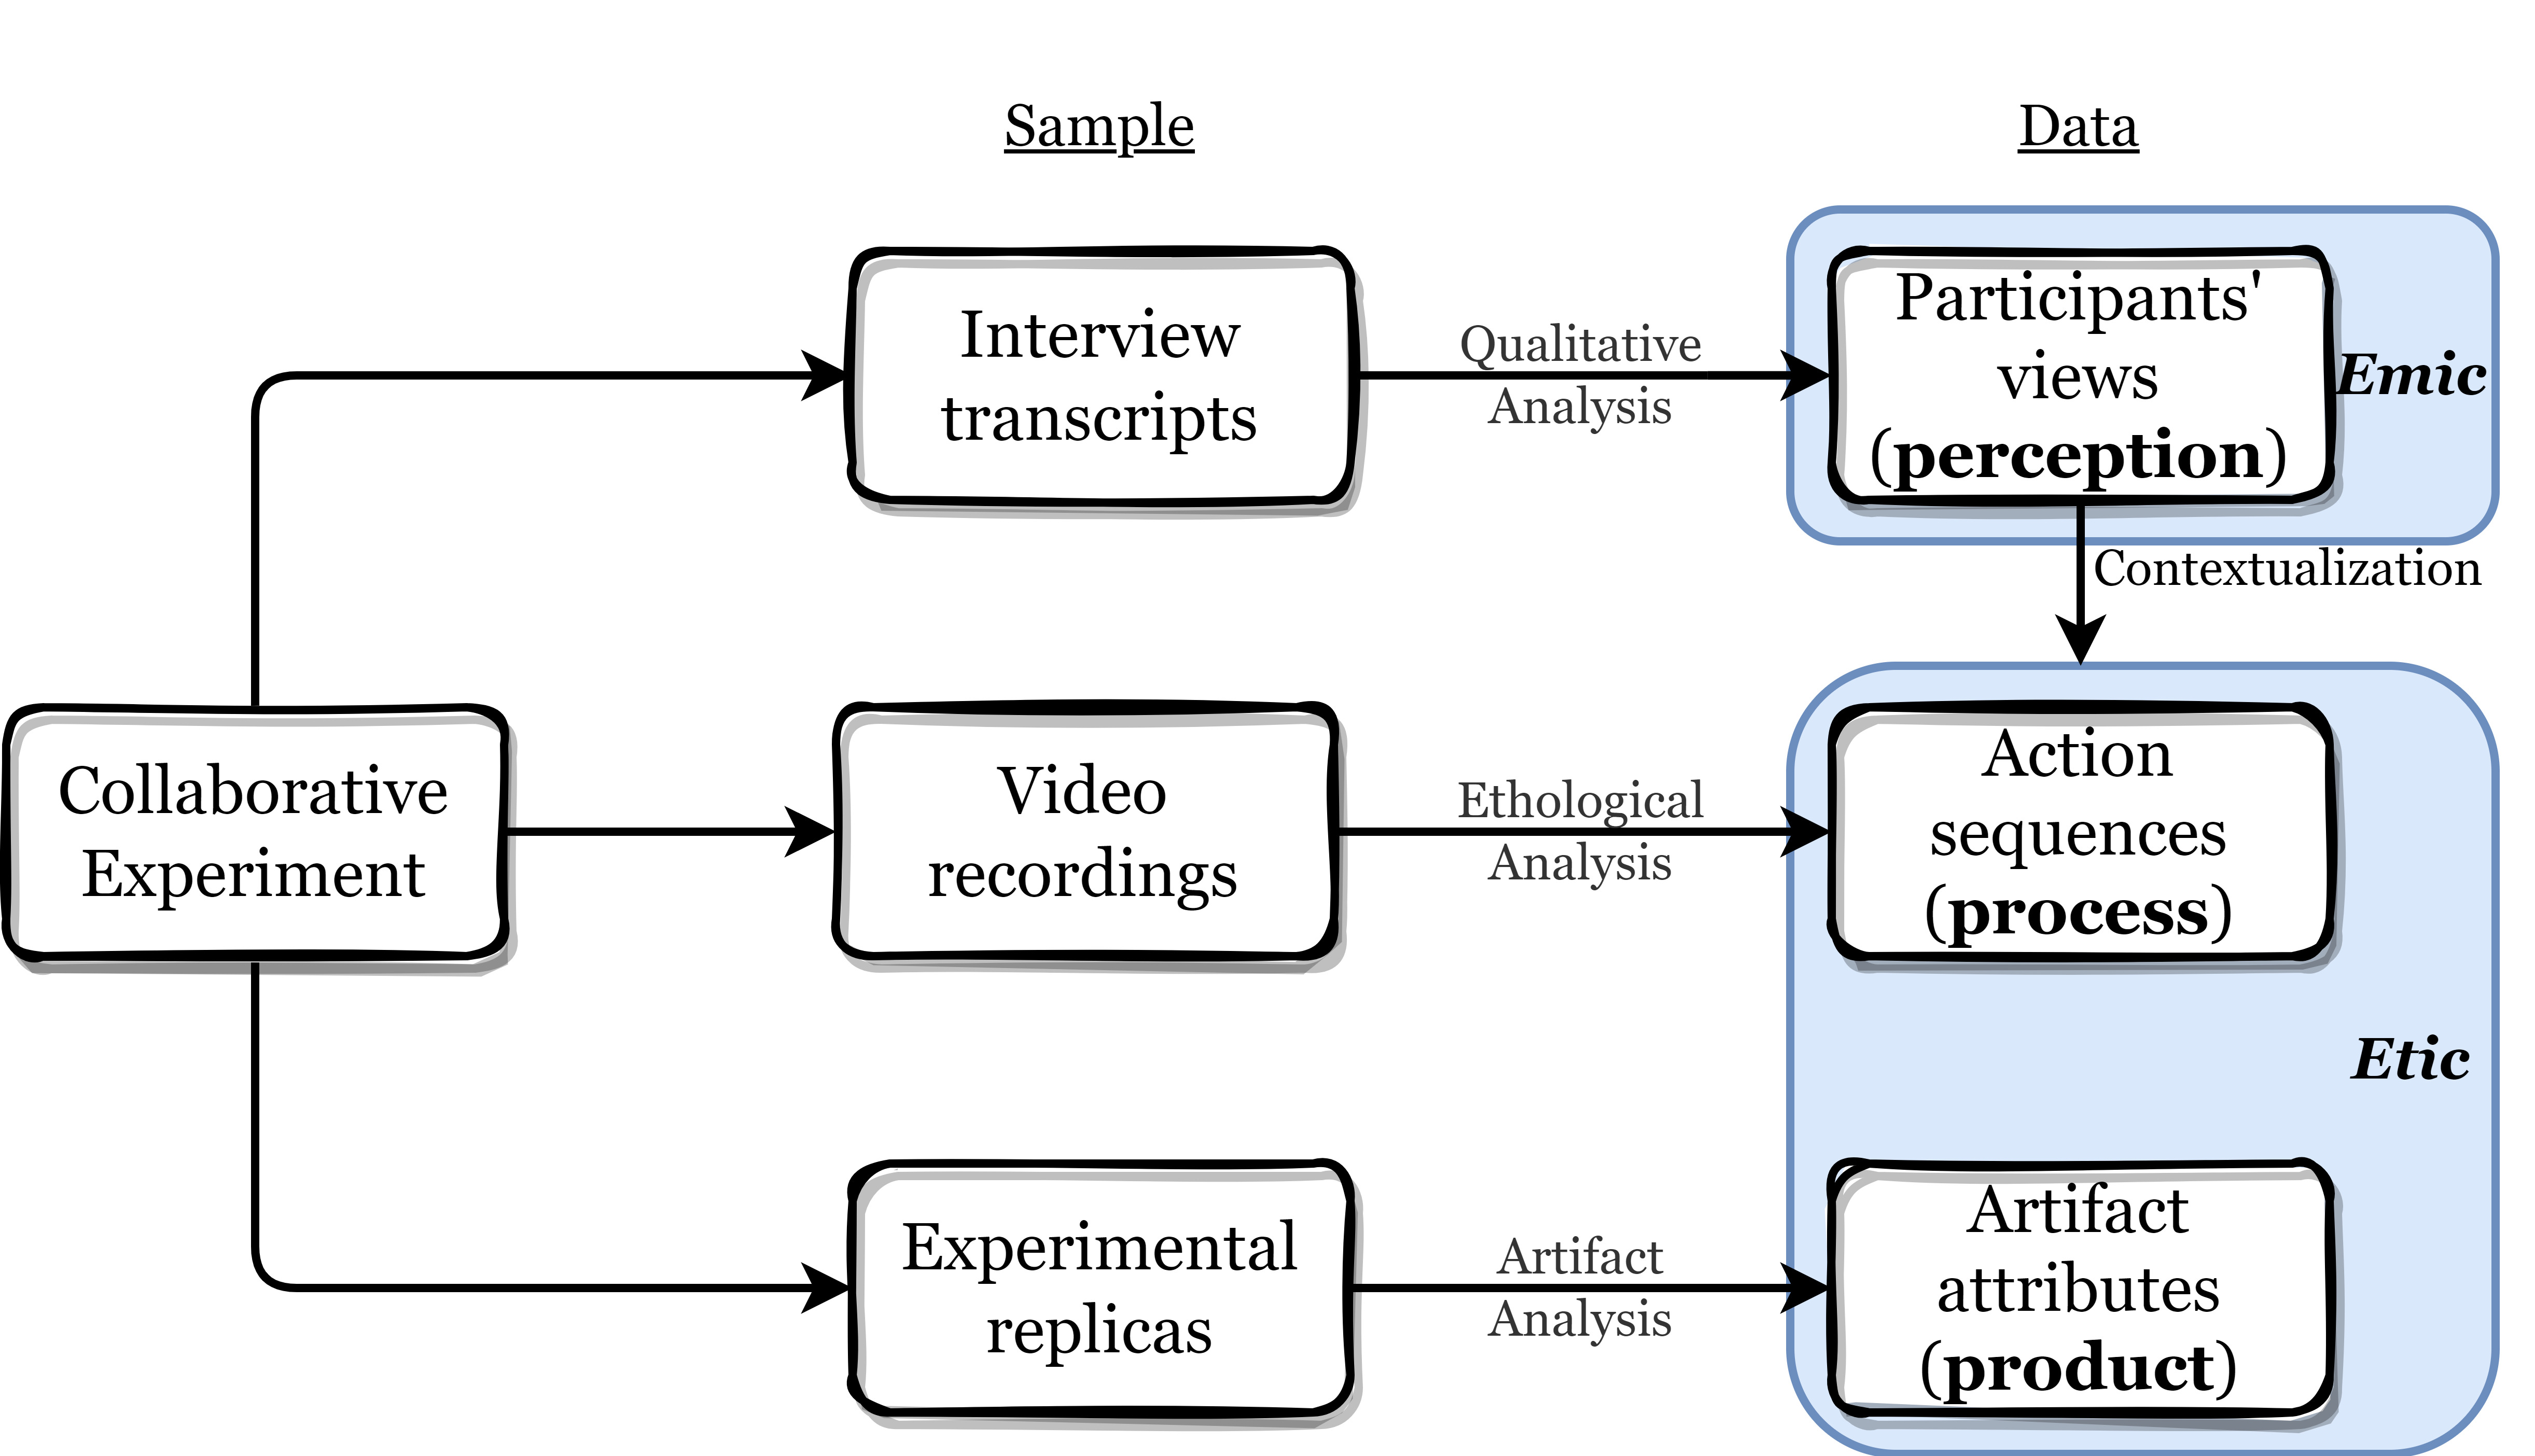
\includegraphics[width=0.8\textwidth,height=\textheight]{../figure/Fig1.jpg}

}

\caption{A schematic diagram demonstrating how to operationalize the
Perception-Process-Product conceptual framework.}

\end{figure}%

\subsection{Product-level data}\label{product-level-data}

Traditionally speaking, the product-level data, namely the documentation
and analysis of replicas, form the sole research subject of experimental
archaeology and serve as the tangible foundation for analogical
inference in the interpretation of archaeological materials. It can
exist in the form of spreadsheets containing detailed technological
attributes, photos and illustrations, or high-resolution 3D scans of
individual artifacts or a whole assemblage. No particular modification
regarding the collection procedure of product-level data is required in
the context of the Triple P framework, although the definition of
variables measured and the documentation techniques (models of
camera/scanners, light setting, processing software version and
workflow, etc.) should be always available in the relevant meta-data. I
also strongly recommend adopting good habits in spreadsheet data
organization (\citeproc{ref-broman2018}{Broman \& Woo, 2018}).

\subsection{Process-level data}\label{process-level-data}

While systematic behavioral coding methods widely used in the study of
non-human animal behavior (\citeproc{ref-fragaszy2018}{Fragaszy \&
Mangalam, 2018}) are still largely neglected among archaeologists,
attempts to reconstruct behavioral sequences involved in the manufacture
of material remains are not infrequent, ranging from the
well-established chaîne opératoire approach
(\citeproc{ref-audouze2017}{Audouze et al., 2017};
\citeproc{ref-delage2017}{Delage, 2017};
\citeproc{ref-dobres1999}{Dobres, 1999};
\citeproc{ref-porqueddu2023}{Porqueddu et al., 2023};
\citeproc{ref-soressi2011}{Soressi \& Geneste, 2011}) to the more recent
cognigram method. To illustrate the benefits and drawbacks of existing
analytical frameworks, here I will use the cognigram as an example,
which was first systematically developed and applied in archaeological
research by Haidle (\citeproc{ref-haidleHowThinkSimple2009}{Haidle,
2009}, \citeproc{ref-haidle2010}{2010}, \citeproc{ref-haidle2014}{2014},
\citeproc{ref-haidle2023}{2023}). A cognigram is a graphical
representation of the reconstructed behavior behind archaeological
artifacts in chronological order of appearance
(\citeproc{ref-haidle2014}{Haidle, 2014}), which essentially represents
an abstracting process of a series of action sequences achieving a
similar goal. This approach provides an elegant descriptive methodology
yet is limited by its normative and analytical orientation, meaning it
cannot handle variation very well. To some extent, it describes the
minimal steps to achieve a goal from the perspective of reverse
engineering and reflects the analyst's own causal understanding.
However, this may be biased because 1) certain causal insights in stone
fracture mechanics remain opaque to academic knappers until they are
revealed through controlled experiments by Dibble and his colleagues
(\citeproc{ref-li2022}{Li et al., 2022}) 2) ethnographic studies
demonstrated that expert non-academic practitioners can have a different
set of causal understanding (\citeproc{ref-harris2021}{Harris et al.,
2021}).

Consequently, we need to accumulate more real-world data by recording a
large number of toolmaking videos and conducting systematic ethogram
analysis. With the emergence of new software platforms such as BORIS
(\citeproc{ref-friard2016}{Friard \& Gamba, 2016}), the difficulty of
coding has decreased significantly in recent years (\textbf{Figure}
@ref(fig:ethogram)). Here I use a modified version of action grammar
developed by (\citeproc{ref-stout2021}{Stout et al., 2021}) as an
example, among multiple coding schemes featuring different research
focus (\citeproc{ref-muller2023}{Muller et al., 2023}) or granularity
(\citeproc{ref-cueva-temprana2019}{Cueva-Temprana et al., 2019};
\citeproc{ref-mahaney2014}{Mahaney, 2014}; \citeproc{ref-roux2005}{Roux
\& David, 2005}). The knapping action recorded in videos can be coded
following the ethogram presented in \textbf{Table} @ref(tab:tab1).
Depending on the original research question, sequences of coded actions
can then be used in further analysis, such as the measurement of
complexity of various technological systems, a classical topic in
paleolithic archaeology and the evolution of human cognition
(\citeproc{ref-muller2017}{Muller et al., 2017};
\citeproc{ref-perreault2013}{Perreault et al., 2013}). Unlike the
traditional approaches resorting to the extraction and comparison of
lithic attributes, Stout et al. (\citeproc{ref-stout2021}{2021})
recorded the videos of expert flintknappers reproducing Oldowan and
Acheulean technologies and then manually parsed their knapping
activities using action grammar, generating multiple sequences of
actions. Borrowing tools from computational linguistics, they then
calculated the transition probability between each action category
across two technological systems, which provided an objective and
quantifiable proxy of measuring technological complexity. Another
scenario of its application is the measurement of behavioral similarity
across individuals (\citeproc{ref-cristino2010}{Cristino et al., 2010};
\citeproc{ref-mobbs2021}{Mobbs et al., 2021}), which is particularly
relevant in the above-mentioned cultural transmission experiments.
Again, since the existing works in this topic mainly focuses on the sole
analysis of experimental replicas, many aspects of knapping skill
learning processes remain unclear. For example, how do different
individual learning strategies (high-fidelity action copying
vs.~predominantly trial-and-error learning) affect the morphological
variation of their final products? Or will learning behavioral
conformity within a community of practice necessarily lead to the
homogeneity in the formation of lithic assemblages? To answer these
questions, the quantitative analysis of process-level data associated
with the product-level data become necessary. Behatrix
(\url{https://www.boris.unito.it/behatrix/}), a sister software of
BORIS, allows us to calculate the action sequence (dis)similarity
between novice learners and expert demonstrators/fellow novice learners
using established algorithms (see \citeproc{ref-cordoni2022}{Cordoni et
al., 2022} for an application of analyzing play behavior similarity
among gorillas).

\begin{figure}[H]

{\centering 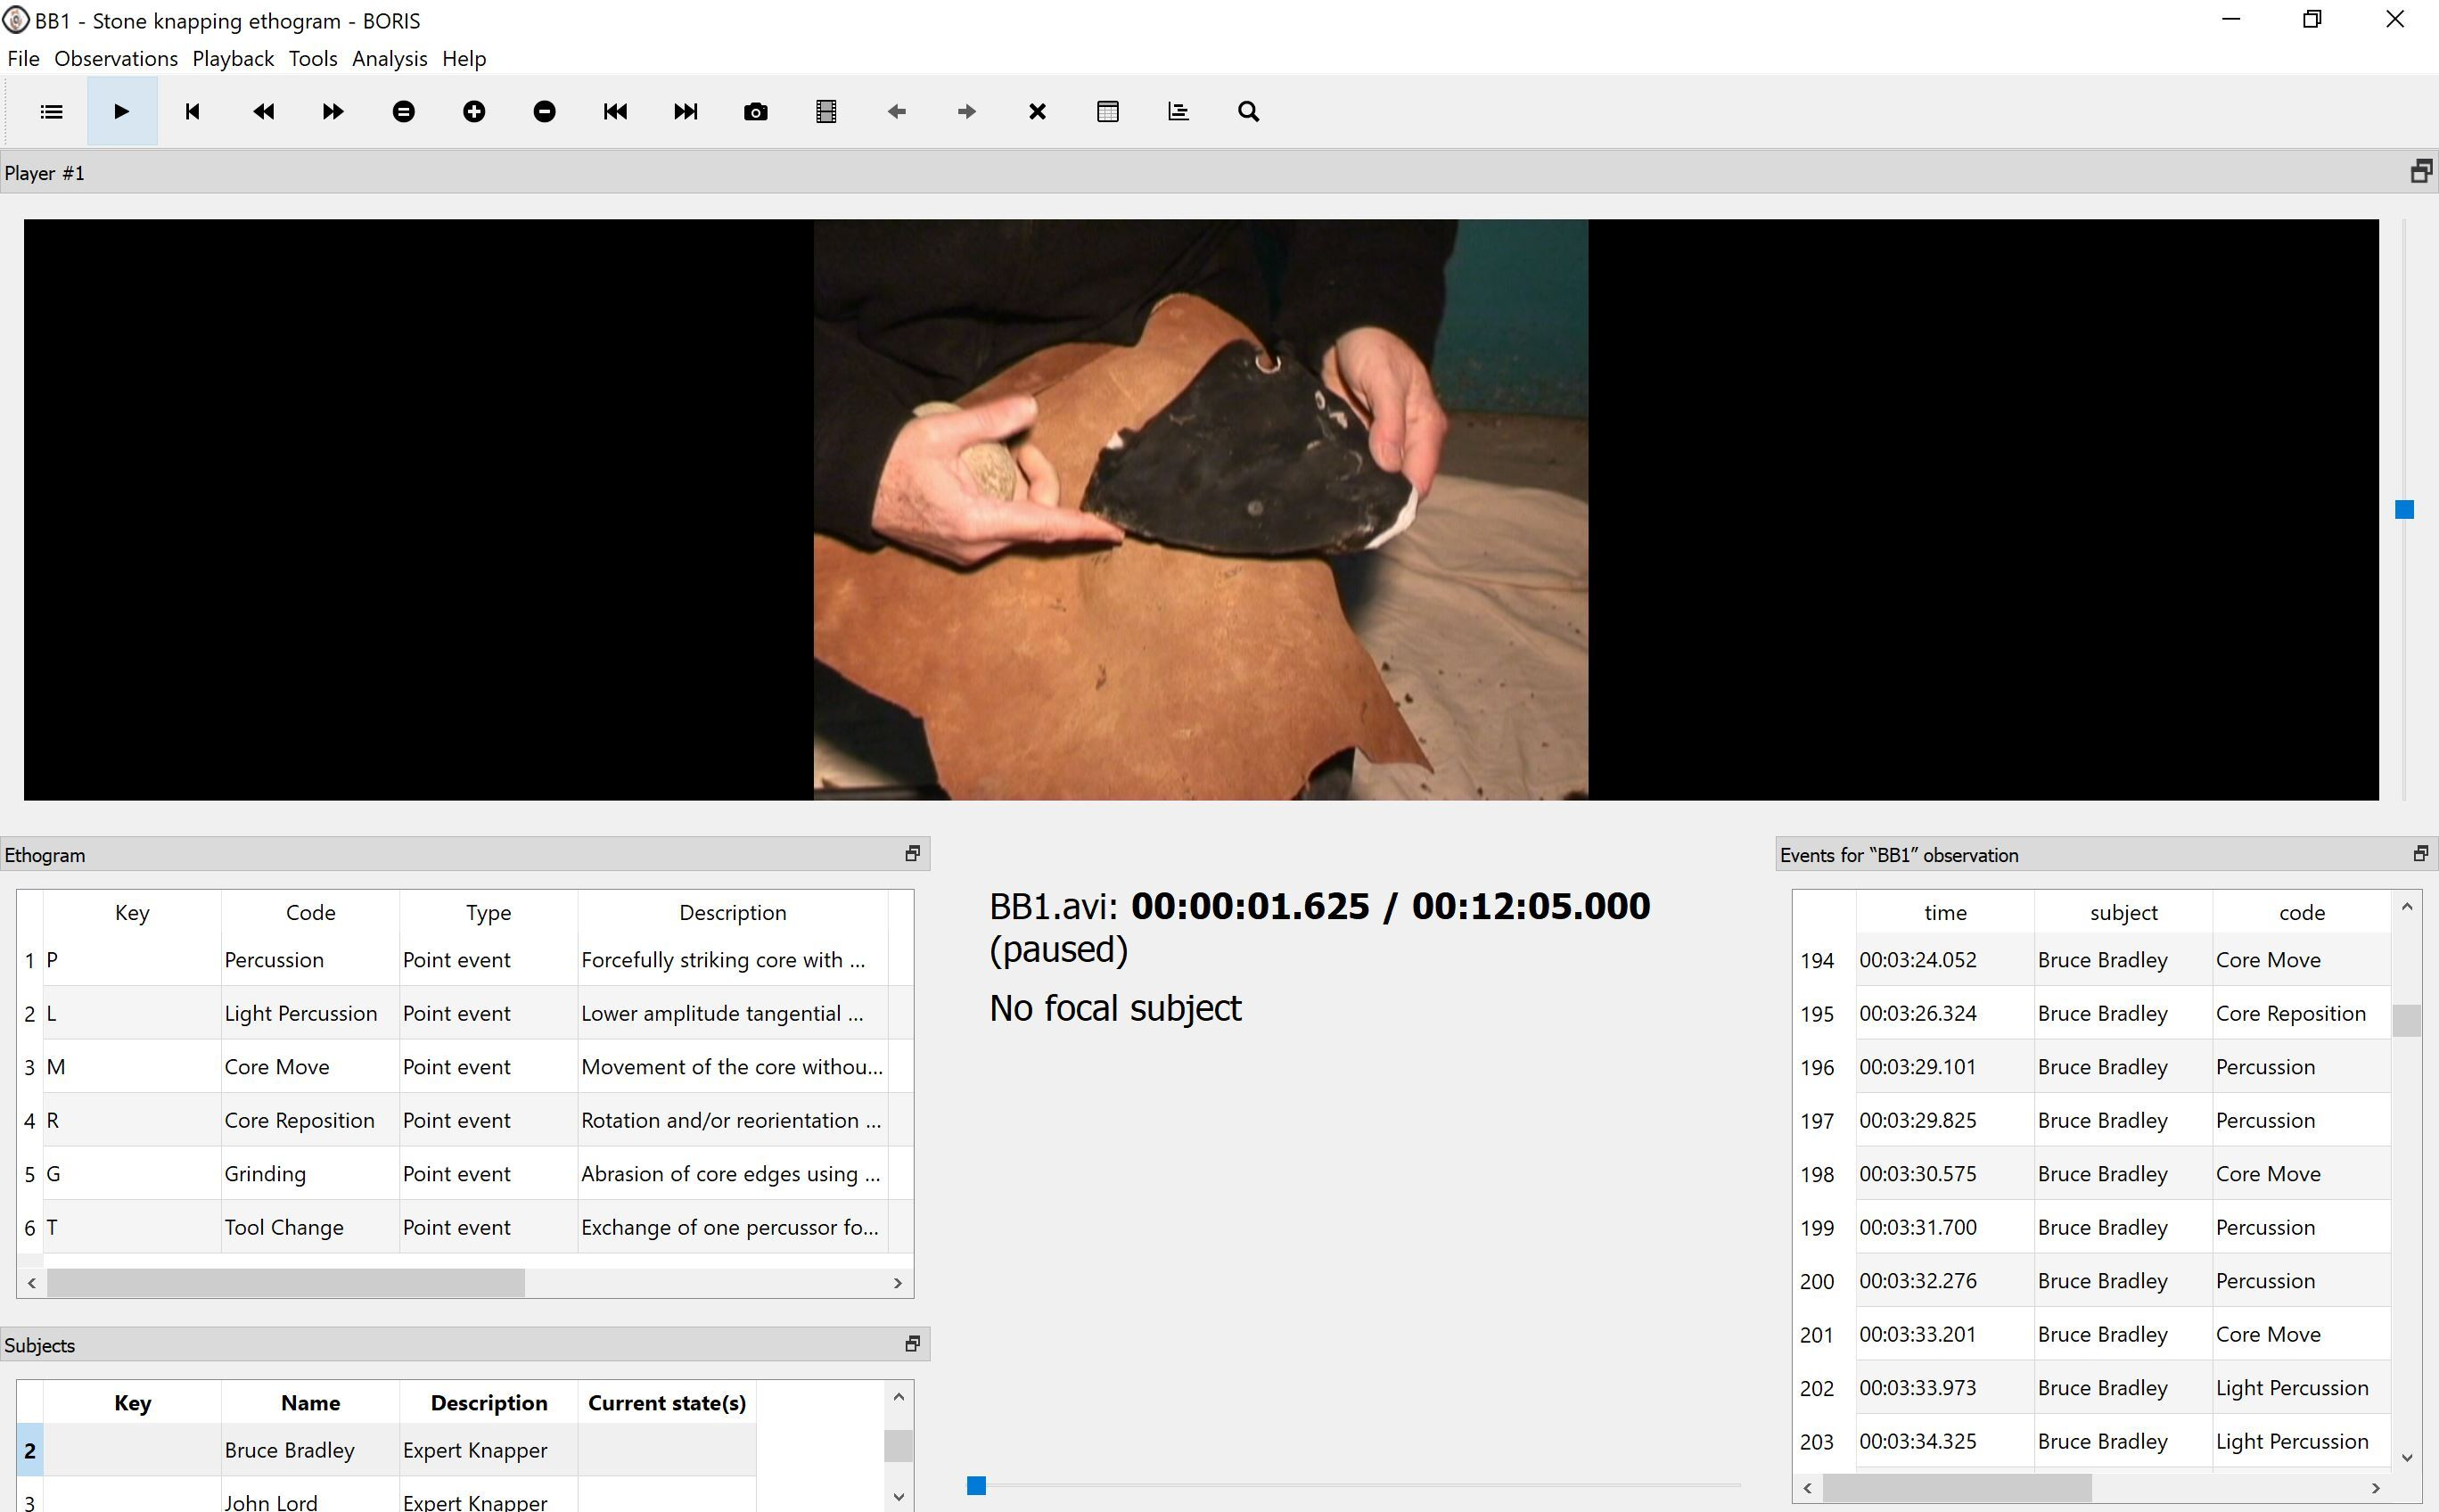
\includegraphics[width=1\textwidth,height=\textheight]{../figure/Fig2.jpg}

}

\caption{An example of coding a handaxe knapping session using the BORIS
software.}

\end{figure}%

\begin{longtable}[]{@{}
  >{\raggedright\arraybackslash}p{(\columnwidth - 2\tabcolsep) * \real{0.0914}}
  >{\raggedright\arraybackslash}p{(\columnwidth - 2\tabcolsep) * \real{0.9086}}@{}}
\caption{A modified version of the original action grammar presented in
(\citeproc{ref-stout2021}{Stout et al., 2021})}\tabularnewline
\toprule\noalign{}
\begin{minipage}[b]{\linewidth}\raggedright
Action
\end{minipage} & \begin{minipage}[b]{\linewidth}\raggedright
Definition
\end{minipage} \\
\midrule\noalign{}
\endfirsthead
\toprule\noalign{}
\begin{minipage}[b]{\linewidth}\raggedright
Action
\end{minipage} & \begin{minipage}[b]{\linewidth}\raggedright
Definition
\end{minipage} \\
\midrule\noalign{}
\endhead
\bottomrule\noalign{}
\endlastfoot
Percussion & Forcefully striking core with percussor (hammerstone or
antler billet) in such a way as to potentially remove a flake. Each
strike should be counted as a single action. \\
Light Percussion & Lower amplitude tangential strike to the tool edge of
the kind often employed for platform preparation. Each strike should be
counted as a single action. \\
Core Move & Movement of the core without a change in grip, which often
occurs during the core inspection \\
Core Reposition & Rotation and/or reorientation of the core involving
repositioning of the hand, which is often associated with the transition
to a new percussion target \\
Grinding & Abrasion of core edges using a hammerstone. The abrasion
movement should come from at least two different directions. \\
Tool Change & Exchange of one percussor for another \\
Winding Up & Preparational percussor movements towards the core that do
not lead to the detachment of flakes, which can either be in direct
contact with cores or not. \\
\end{longtable}

\subsection{Perception-level data}\label{perception-level-data}

Ethnographies revolving around experimental archaeology as a field
(\citeproc{ref-reevesflores2012}{Reeves Flores, 2012}), as well as
practices of specific technologies like flintknapping, including
contemporary U.S. hobbyists (\citeproc{ref-whittaker2004}{Whittaker,
2004}) and knapping practitioners in various non-industrial societies
(\citeproc{ref-arthur2018}{Arthur, 2018};
\citeproc{ref-stout2002}{Stout, 2002}), are far from novel. However,
ethnography has never been formally recognized as a legitimate research
method in mainstream experimental archaeology. Echoing with the recent
trends of adopting embodied cognition (\citeproc{ref-varela2017}{Varela
et al., 2017}) in archaeological research
(\citeproc{ref-malafouris2013}{Malafouris, 2013}), ethnographic data and
methods can reveal hidden information (e.g., intention, phenomenology)
that is otherwise irretrievable and thus should occupy a unique niche in
experimental archaeology. Within the broader context of burgeoning
interest in mixed-method research in contemporary social science
(\citeproc{ref-creswell2017}{Creswell \& Clark, 2017}), this also echoes
the post-positivist turn in psychology in the past decades, particularly
the emphasis on the value of incorporating qualitative research
(\citeproc{ref-stoutCognitiveScienceTechnology2021}{Stout, 2021};
\citeproc{ref-syed2022}{Syed \& McLean, 2022};
\citeproc{ref-weger2019}{Weger et al., 2019}).

Through participant observation, interviews, and detailed field notes,
ethnography can capture the subtle nuances of perception, such as
cognitive affordances (\citeproc{ref-hussain2021}{Hussain \& Will,
2021}; \citeproc{ref-roepstorff2008}{Roepstorff, 2008}), sensory
experiences (\citeproc{ref-day2013}{Day, 2013};
\citeproc{ref-oneill2019}{O'Neill \& O'Sullivan, 2019};
\citeproc{ref-therout2019}{Skeates \& Day, 2019}), social interactions,
and cultural meanings associated with the experimental activities
(\citeproc{ref-gowlland2019}{Gowlland, 2019}). Compared with the
ethological methods, the interview questions and participant observation
in ethnographic methods feature an even higher degree of freedom and
rely more heavily on the research question as well as ad-hoc
interaction. One potential application of ethnographic methods in
experimental archaeology of stone artifacts is asking knappers about the
intentions of each action and see how it matches with the results as
revealed by lithic analysis of replicas, which can provide crucial
contextual information addressing the issues of equifinality and
multifinality in the formation of lithic assemblage. For example, serial
formation of step-fracture on the debitage surface are commonly
interpreted as unintentional mistakes indicative of novice knappers,
while in some cases researchers treat it as evidence of deliberate core
rejuvenation (\citeproc{ref-akerman1993}{Akerman, 1993}: 126). The
accumulation of testimonies by participating knappers in terms of their
intended outcome become useful in this scenario, although these
materials should be examined in combination with the relevant product-
and process-level data in a careful manner. Instead of seeing intention
as something abstruse or unapproachable in archaeology
(\citeproc{ref-david2004}{David, 2004};
\citeproc{ref-russell2004}{Russell, 2004}), the Triple P framework
adopts a novel definition proposed by Quillien and German
(\citeproc{ref-quillien2021}{2021}: 1) from the perspective of causal
perception, namely ``an agent did X \emph{intentionally} to the extent
that X was causally dependent on how much the agent wanted X to happen
(or not to happen).'' In this sense, the mismatch between how different
individuals perceive cause-and-effect relationships and how they are
organized according to physical laws is exactly where interesting
variation emerges and where ethnography becomes necessary.

\subsection{Multi-level sample and data
curation}\label{multi-level-sample-and-data-curation}

The comparative study and large-scale synthesis of variation data
require the building of centralized, open-access, and carefully curated
data infrastructure (\citeproc{ref-marwick2018}{Marwick \& Birch,
2018}), which unfortunately still does not exist yet in experimental
archaeology. The accessibility and availability of experimental data can
foster collaboration and enhance the reproducibility and transparency of
research findings, as others can verify and validate the results by
examining the original data. Moreover, a centralized database also
promotes data preservation and long-term accessibility. By storing
experimental data in a structured and organized manner, it safeguards
valuable information from potential loss or degradation over time. This
preservation ensures that the data remains accessible for future
researchers, avoiding the loss of valuable insights and preventing the
need for redundant and costly repetitions of experiments. It also allows
for the reanalysis of existing data, facilitating discoveries and
insights that may not have been initially anticipated. However, it has
been widely acknowledged that the reuse of archaeological data has not
received enough attention among researchers in our discipline
(\citeproc{ref-faniel2018}{Faniel et al., 2018};
\citeproc{ref-huggett2018}{Huggett, 2018};
\citeproc{ref-moody2021}{Moody et al., 2021}).

Among the three dimensions of the Triple P framework, the product-level
data are usually stored in the format of spreadsheets, photos, and 3D
models, and the perception-level data formats mainly include audio files
and their transcribed texts, whereas videos are the main vector of
process-level data, a rather non-traditional data format in
archaeological research featuring the largest file size compared with
the other two. As such, following data sharing principles of FAIR
(\citeproc{ref-wilkinson2016}{Wilkinson et al., 2016}) and CARE
(\citeproc{ref-carroll2020}{Carroll et al., 2020}), the Triple P
framework recommends Databrary (\citeproc{ref-gilmore2015}{Gilmore et
al., 2015}; \citeproc{ref-simon2015}{Simon et al., 2015}), a web-based
library originally designed for developmental scientists, as the main
data curation platform, where researchers can freely upload video files
with no size limit and related metadata that can connect with different
types of data within the same project. Databrary has three advantages
compared with other data storage solutions: a) no cost from the side of
researchers; 2) long-term data security monitored by a specialized
maintenance team; and 3) fostering potential collaborations between
experimental archaeologists and developmental psychologists.

On top of the digital data curation, an easily ignored but crucial
aspect regarding the integrity and reliability of research in
experimental archaeology is the long-term and proper curation of
psychical specimens produced during experiments, which is particularly
relevant to the product-level data. Haythron et al.
(\citeproc{ref-haythorn2018}{2018}) sharply pointed out that re-running
statistical analyses on a publicly available spreadsheet containing
incorrect lithic projectile attribute data would be meaningless. In this
case, reexamination of the actual experiment samples become necessary.
Moreover, it is likely that new research questions can only be answered
through direct observation and measurement of the experimental
assemblages themselves but not available in previously recorded data
sets (\citeproc{ref-eren2016}{Eren et al., 2016}). The existence of
these possibilities thus require that an experimental assemblage of
interest should be ideally curated in public institutions with easy
access, granting that their contextual information is still properly
preserved (\citeproc{ref-haythorn2018}{Haythorn et al., 2018}).

\section{Conclusion}\label{conclusion}

Through the broadening of traditional data types and recording methods
revolving around experimental replicas \emph{per se}, the Triple P
conceptual framework allows the amplified multiscale expression of
material cultural variation. It is also compatible with many theoretical
orientations, ranging from behavioral archaeology (emphasis on video
recording of behavioral processes) through evolutionary archaeology
(emphasis on the amplification of variation) to post-processual
archaeology (emphasis on perception through ethnography). In terms of
its research practice, it embraces a collaborative mode of knowledge
production by involving a more diverse pool of stakeholders. It should
be noted that this alternative mode of knowledge production is not
necessarily a bundle sale, where each single component is independent
and detachable according to the individual research question. Instead,
it can serve as a heuristic tool to inspire potential readers to explore
a broader range of data collection and analysis strategies. To
summarize, the innovativeness, flexibility, and inclusiveness of the
Triple P conceptual framework have enormous potential in redefining what
can be and what should be studied by experimental archaeology as a field
and thereby contributing to a better understanding of our deep past.

\section{Acknowledgments}\label{acknowledgments}

I thank Dietrich Stout for his helpful comments on earlier drafts of
this article as well as Mark Moore and Shaya Jannati for inspiring
discussions. I am also grateful for Metin Eren and two other anonymous
reviewers for their insightful feedback. This study was supported by the
Leakey Foundation research grant titled ``Inferring skill reproduction
from stone artifacts: A middle‐range approach'' as well as the
International Society of Human Ethology's Owen Aldis Award project
titled ``Sealed in stones: The computational ethology of stone
toolmaking and its implications to the evolution of cultural
transmission.''

\section*{References}\label{references}
\addcontentsline{toc}{section}{References}

\phantomsection\label{refs}
\begin{CSLReferences}{1}{0}
\bibitem[\citeproctext]{ref-acerbi2009}
Acerbi, A., Enquist, M., \& Ghirlanda, S. (2009). Cultural evolution and
individual development of openness and conservatism. \emph{Proceedings
of the National Academy of Sciences}, \emph{106}(45), 18931--18935.
\url{https://doi.org/10.1073/pnas.0908889106}

\bibitem[\citeproctext]{ref-akerman1993}
Akerman, K. (1993). The status of the horsehoof core. \emph{Records of
the Australian Museum, Supplement}, \emph{17}, 125127.
\url{https://media.australian.museum/media/Uploads/Journals/17795/64_complete.pdf}

\bibitem[\citeproctext]{ref-almaatouq2024}
Almaatouq, A., Griffiths, T. L., Suchow, J. W., Whiting, M. E., Evans,
J., \& Watts, D. J. (2024). Beyond playing 20 questions with nature:
Integrative experiment design in the social and behavioral sciences.
\emph{Behavioral and Brain Sciences}, \emph{47}, e33.
\url{https://doi.org/10.1017/S0140525X22002874}

\bibitem[\citeproctext]{ref-antuxf3n2017}
Antón, S. C., \& Kuzawa, C. W. (2017). Early homo, plasticity and the
extended evolutionary synthesis. \emph{Interface Focus}, \emph{7}(5),
20170004. \url{https://doi.org/10.1098/rsfs.2017.0004}

\bibitem[\citeproctext]{ref-apicella2020}
Apicella, C., Norenzayan, A., \& Henrich, J. (2020). Beyond WEIRD: A
review of the last decade and a look ahead to the global laboratory of
the future. \emph{Evolution and Human Behavior}, \emph{41}(5), 319--329.
\url{https://doi.org/10.1016/j.evolhumbehav.2020.07.015}

\bibitem[\citeproctext]{ref-arthur2018}
Arthur, K. W. (2018). \emph{The lives of stone tools: Crafting the
status, skill, and identity of flintknappers}. University of Arizona
Press.

\bibitem[\citeproctext]{ref-arthur2021}
Arthur, K. W. (2021). Material Scientists: Learning the Importance of
Colour and Brightness from Lithic Practitioners. \emph{Cambridge
Archaeological Journal}, \emph{31}(2), 293--304.
\url{https://doi.org/10.1017/S0959774320000347}

\bibitem[\citeproctext]{ref-arthur2024}
Arthur, K. W., Barkai, R., Allen, C., Shpayer, E. A., Efrati, B.,
Finkel, M., Ganchrow, D., Horowitz, R. A., Litov, V., Lombard, M.,
Sillitoe, P., \& Swenson, E. (2024). Ancestral Stones and Stone Stories:
Reimagining Human Relationships with Stone from the Paleolithic to the
Present. \emph{Archaeologies}, \emph{20}(1), 1--23.
\url{https://doi.org/10.1007/s11759-024-09502-y}

\bibitem[\citeproctext]{ref-atalay2012}
Atalay, S. (2012). \emph{Community-based archaeology: Research with, by,
and for indigenous and local communities}. University of California
Press.
\url{https://books.google.com/books?hl=en&lr=&id=q7MwDwAAQBAJ&oi=fnd&pg=PR9&dq=sonya+atalay+community+based+archaeology&ots=EoTKMq3e9j&sig=V-q0p0F6b546SQt9lhW7C59Hejw}

\bibitem[\citeproctext]{ref-audouze2017}
Audouze, F., Bodu, P., Karlin, C., Julien, M., Pelegrin, J., \& Perlès,
C. (2017). Leroi-gourhan and the chaîne opératoire: A response to
delage. \emph{World Archaeology}, \emph{49}(5), 718723.
\url{https://doi.org/10.1080/00438243.2017.1416012}

\bibitem[\citeproctext]{ref-barrett2020}
Barrett, H. C. (2020). Towards a Cognitive Science of the Human:
Cross-Cultural Approaches and Their Urgency. \emph{Trends in Cognitive
Sciences}, \emph{24}(8), 620--638.
\url{https://doi.org/10.1016/j.tics.2020.05.007}

\bibitem[\citeproctext]{ref-batalla2016}
Batalla, A. N. (2016). Studies of indigenous lithic procurement in
Uruguay and their implications for Southern Cone archaeology.
\emph{Journal of Lithic Studies}, \emph{3}(1), 265--292.
\url{https://doi.org/10.2218/jls.v3i1.1522}

\bibitem[\citeproctext]{ref-bell2014}
Bell, M. (2014). \emph{Experimental archaeology at the crossroads: A
contribution to interpretation or evidence of {`}xeroxing{'}?} (R.
Chapman \& A. Wylie, Eds.; pp. 42--58). Routledge.

\bibitem[\citeproctext]{ref-berl2015}
Berl, R. E. W., \& Hewlett, B. S. (2015). Cultural Variation in the Use
of Overimitation by the Aka and Ngandu of the Congo Basin. \emph{PLOS
ONE}, \emph{10}(3), e0120180.
\url{https://doi.org/10.1371/journal.pone.0120180}

\bibitem[\citeproctext]{ref-bettinger1982}
Bettinger, R. L., \& Baumhoff, M. A. (1982). The Numic Spread: Great
Basin Cultures in Competition. \emph{American Antiquity}, \emph{47}(3),
485--503. \url{https://doi.org/10.2307/280231}

\bibitem[\citeproctext]{ref-blessing2021}
Blessing, M. A., \& Schmidt, P. (2021). On the efficiency of
palaeolithic birch tar making. \emph{Journal of Archaeological Science:
Reports}, \emph{38}, 103096.
\url{https://doi.org/10.1016/j.jasrep.2021.103096}

\bibitem[\citeproctext]{ref-broman2018}
Broman, K. W., \& Woo, K. H. (2018). Data organization in spreadsheets.
\emph{The American Statistician}, \emph{72}(1), 2--10.
\url{https://doi.org/10.1080/00031305.2017.1375989}

\bibitem[\citeproctext]{ref-carroll2020}
Carroll, S. R., Garba, I., Figueroa-Rodríguez, O. L., Holbrook, J.,
Lovett, R., Materechera, S., Parsons, M., Raseroka, K.,
Rodriguez-Lonebear, D., Rowe, R., Sara, R., Walker, J. D., Anderson, J.,
\& Hudson, M. (2020). The CARE Principles for Indigenous Data
Governance. \emph{Data Science Journal}, \emph{19}(1), 43.
\url{https://doi.org/10.5334/dsj-2020-043}

\bibitem[\citeproctext]{ref-clay2018}
Clay, Z., \& Tennie, C. (2018). Is Overimitation a Uniquely Human
Phenomenon? Insights From Human Children as Compared to Bonobos.
\emph{Child Development}, \emph{89}(5), 1535--1544.
\url{https://doi.org/10.1111/cdev.12857}

\bibitem[\citeproctext]{ref-coles1979}
Coles, J. M. (1979). \emph{Experimental archaeology}. Academic Press.

\bibitem[\citeproctext]{ref-conrad2023}
Conrad, G., Hough, S., Baldino, J., Gala, N., Buchanan, B., Walker, R.
S., Key, A., Redmond, B. G., Bebber, M. R., \& Eren, M. I. (2023).
Clovis bone versus stone weapon tip penetration: Thinking about relative
costs and benefits, experimental assumptions, and archaeological
unknowns at sheriden cave, ohio, u.s.a. \emph{Journal of Archaeological
Science: Reports}, \emph{52}, 104295.
\url{https://doi.org/10.1016/j.jasrep.2023.104295}

\bibitem[\citeproctext]{ref-cordoni2022}
Cordoni, G., Pirarba, L., Elies, S., Demuru, E., Guéry, J.-P., \&
Norscia, I. (2022). Adult{\textendash}adult play in captive lowland
gorillas (Gorilla gorilla gorilla). \emph{Primates}, \emph{63}(3),
225--235. \url{https://doi.org/10.1007/s10329-022-00973-7}

\bibitem[\citeproctext]{ref-crabtree1977}
Crabtree, D. E. (1977). \emph{The obtuse angle as a functional edge} (D.
Ingersoll, J. E. Yellen, \& W. MacDonald, Eds.; pp. 38--51). Columbia
University Press.

\bibitem[\citeproctext]{ref-creswell2017}
Creswell, J. W., \& Clark, V. L. P. (2017). \emph{Designing and
conducting mixed methods research} (3rd edition). SAGE Publications,
Inc.

\bibitem[\citeproctext]{ref-cristino2010}
Cristino, F., Mathôt, S., Theeuwes, J., \& Gilchrist, I. D. (2010).
ScanMatch: A novel method for comparing fixation sequences.
\emph{Behavior Research Methods}, \emph{42}(3), 692--700.
\url{https://doi.org/10.3758/BRM.42.3.692}

\bibitem[\citeproctext]{ref-cueva-temprana2019}
Cueva-Temprana, A., Lombao, D., Morales, J. I., Geribàs, N., \&
Mosquera, M. (2019). Gestures during knapping: A two-perspective
approach to pleistocene technologies. \emph{Lithic Technology},
\emph{44}(2), 74--89.
\url{https://doi.org/10.1080/01977261.2019.1587255}

\bibitem[\citeproctext]{ref-cunningham2021}
Cunningham, S. (2021). \emph{Causal inference: The mixtape}. Yale
University Press. \url{https://doi.org/10.2307/j.ctv1c29t27}

\bibitem[\citeproctext]{ref-currie2022}
Currie, A. (2022). Speculation Made Material: Experimental Archaeology
and Maker{'}s Knowledge. \emph{Philosophy of Science}, \emph{89}(2),
337--359. \url{https://doi.org/10.1017/psa.2021.31}

\bibitem[\citeproctext]{ref-david2004}
David, B. (2004). Intentionality, Agency and an Archaeology of Choice.
\emph{Cambridge Archaeological Journal}, \emph{14}(1), 67--71.
\url{https://doi.org/10.1017/S0959774304220054}

\bibitem[\citeproctext]{ref-day2013}
Day, J. (2013). \emph{Making senses of the past: Toward a sensory
archaeology}. Southern Illinois University Press.
\url{https://muse.jhu.edu/pub/186/monograph/book/23997}

\bibitem[\citeproctext]{ref-delage2017}
Delage, C. (2017). Once upon a time{\ldots{}}the (hi)story of the
concept of the chaîne opératoire in french prehistory. \emph{World
Archaeology}, \emph{49}(2), 158173.
\url{https://doi.org/10.1080/00438243.2017.1300104}

\bibitem[\citeproctext]{ref-dobres1999}
Dobres, M.-A. (1999). \emph{Technology{'}s links and chaînes: The
processual unfolding of technique and technician} (D. Marcia-Anne \& C.
R. Hoffman, Eds.; p. 124146). Smithsonian Institution Press.
\url{http://ww.plndp.org/Departments/Joukowsky_Institute/courses/archaeologicaltheory/files/3787748.pdf}

\bibitem[\citeproctext]{ref-domuxednguez-rodrigo2008}
Domínguez-Rodrigo, M. (2008). Conceptual premises in experimental design
and their bearing on the use of analogy: An example from experiments on
cut marks. \emph{World Archaeology}, \emph{40}(1), 67--82.
\url{https://doi.org/10.1080/00438240701843629}

\bibitem[\citeproctext]{ref-douglass2020}
Douglass, K. (2020). Amy ty lilin-draza{'}ay: Building Archaeological
Practice on Principles of Community. \emph{African Archaeological
Review}, \emph{37}(3), 481--485.
\url{https://doi.org/10.1007/s10437-020-09404-8}

\bibitem[\citeproctext]{ref-erenExperimentalBisonButchery2024}
Eren, M. I., Bebber, M. R., Mukusha, L., Wilson, M., Boehm, A. R.,
Buchanan, B., Miller, G. L., Skoglund, M., Hayes, J., Barta, M., Bates,
S., Callaghan, R., Floyd, C., Morris, S., Neuharth, S., Newcomb, C.,
Rinella, S., Schneider, C., Smith, M. M., \ldots{} Meltzer, D. J.
(2024). Experimental bison butchery using replica hafted {Clovis} fluted
points and large handheld flakes. \emph{Journal of Archaeological
Science: Reports}, 104480.
\url{https://doi.org/10.1016/j.jasrep.2024.104480}

\bibitem[\citeproctext]{ref-eren2016}
Eren, M. I., Lycett, S. J., Patten, R. J., Buchanan, B., Pargeter, J.,
\& O'Brien, M. J. (2016). Test, model, and method validation: The role
of experimental stone artifact replication in hypothesis-driven
archaeology. \emph{Ethnoarchaeology: Journal of Archaeological,
Ethnographic and Experimental Studies}, \emph{8}(2), 103--136.
\url{https://doi.org/10.1080/19442890.2016.1213972}

\bibitem[\citeproctext]{ref-eren2024}
Eren, M. I., \& Meltzer, D. J. (2024). Controls, conceits, and aiming
for robust inferences in experimental archaeology. \emph{Journal of
Archaeological Science: Reports}, \emph{53}, 104411.
\url{https://doi.org/10.1016/j.jasrep.2024.104411}

\bibitem[\citeproctext]{ref-faniel2018}
Faniel, I. M., Austin, A., Kansa, E., Kansa, S. W., France, P., Jacobs,
J., Boytner, R., \& Yakel, E. (2018). Beyond the Archive: Bridging Data
Creation and Reuse in Archaeology. \emph{Advances in Archaeological
Practice}, \emph{6}(2), 105--116.
\url{https://doi.org/10.1017/aap.2018.2}

\bibitem[\citeproctext]{ref-flenniken1984}
Flenniken, J. J. (1984). The past, present, and future of flintknapping:
An anthropological perspective. \emph{Annual Review of Anthropology},
\emph{13}(1), 187--203.
\url{https://doi.org/10.1146/annurev.an.13.100184.001155}

\bibitem[\citeproctext]{ref-fragaszy2018}
Fragaszy, D. M., \& Mangalam, M. (2018). \emph{Chapter Five - Tooling}
(M. Naguib, L. Barrett, S. D. Healy, J. Podos, L. W. Simmons, \& M. Zuk,
Eds.; Vol. 50, pp. 177--241). Academic Press.
\url{https://doi.org/10.1016/bs.asb.2018.01.001}

\bibitem[\citeproctext]{ref-friard2016}
Friard, O., \& Gamba, M. (2016). BORIS: a free, versatile open-source
event-logging software for video/audio coding and live observations.
\emph{Methods in Ecology and Evolution}, \emph{7}(11), 1325--1330.
\url{https://doi.org/10.1111/2041-210X.12584}

\bibitem[\citeproctext]{ref-gergely2006}
Gergely, G., \& Csibra, G. (2006). \emph{Sylvia's recipe: The role of
imitation and pedagogy in the transmission of cultural knowledge} (S. C.
Levinson \& N. J. Enfield, Eds.; pp. 229--255). Berg Publishers.

\bibitem[\citeproctext]{ref-ghirlanda2006}
Ghirlanda, S., Enquist, M., \& Nakamaru, M. (2006). Cultural evolution
develops its own rules: The rise of conservatism and persuasion.
\emph{Current Anthropology}, \emph{47}(6), 1027--1034.
\url{https://doi.org/10.1086/508696}

\bibitem[\citeproctext]{ref-gilmore2015}
Gilmore, R., Adolph, K., Millman, D., Steiger, L., \& Simon, D. (2015).
Sharing displays and data from vision science research with databrary.
\emph{Journal of Vision}, \emph{15}(12), 280.
\url{https://doi.org/10.1167/15.12.280}

\bibitem[\citeproctext]{ref-gowlland2019}
Gowlland, G. (2019). The sociality of enskilment. \emph{Ethnos},
\emph{84}(3), 508--524.
\url{https://doi.org/10.1080/00141844.2018.1455726}

\bibitem[\citeproctext]{ref-griffin2013}
Griffin, D., Freedman, D. L., Nicholson, B., McConachie, F., \&
Parmington, A. (2013). The koorong project: Experimental archaeology and
wurundjeri continuation of cultural practices. \emph{Excavations,
Surveys and Heritage Management in Victoria}, \emph{2}, 5965.

\bibitem[\citeproctext]{ref-haidleHowThinkSimple2009}
Haidle, M. N. (2009). How to think a simple spear. In S. A. de Beaune,
F. L. Coolidge, \& T. Wynn (Eds.), \emph{Cognitive archaeology and human
evolution} (pp. 57--73). Cambridge University Press.

\bibitem[\citeproctext]{ref-haidle2010}
Haidle, M. N. (2010). Working-memory capacity and the evolution of
modern cognitive potential: Implications from animal and early human
tool use. \emph{Current Anthropology}, \emph{51}(S1), S149--S166.
\url{https://doi.org/10.1086/650295}

\bibitem[\citeproctext]{ref-haidle2014}
Haidle, M. N. (2014). Building a bridge{\textemdash}an archeologist's
perspective on the evolution of causal cognition. \emph{Frontiers in
Psychology}, \emph{5}.
\url{https://www.frontiersin.org/articles/10.3389/fpsyg.2014.01472}

\bibitem[\citeproctext]{ref-haidle2023}
Haidle, M. N. (2023). \emph{Cognigrams: Systematically reconstructing
behavioral architectures as a basis for cognitive archaeology} (T. Wynn,
K. A. Overmann, \& F. L. Coolidge, Eds.; p. C12S1C12S8). Oxford
University Press.
\url{https://doi.org/10.1093/oxfordhb/9780192895950.013.12}

\bibitem[\citeproctext]{ref-harris2021}
Harris, J. A., Boyd, R., \& Wood, B. M. (2021). The role of causal
knowledge in the evolution of traditional technology. \emph{Current
Biology}, \emph{31}(8), 1798--1803.e3.
\url{https://doi.org/10.1016/j.cub.2021.01.096}

\bibitem[\citeproctext]{ref-haythorn2018}
Haythorn, R., Buchanan, B., \& Eren, M. I. (2018). A new look at flaked
stone projectiles from the mixter site (33-ER-4), erie county, ohio,
USA. \emph{Lithic Technology}, \emph{43}(3), 166171.
\url{https://doi.org/10.1080/01977261.2018.1479950}

\bibitem[\citeproctext]{ref-henrichSearchHomoEconomicus2001}
Henrich, J., Boyd, R., Bowles, S., Camerer, C., Fehr, E., Gintis, H., \&
McElreath, R. (2001). In {Search} of {Homo} {Economicus}: {Behavioral}
{Experiments} in 15 {Small}-{Scale} {Societies}. \emph{American Economic
Review}, \emph{91}(2), 73--78. \url{https://doi.org/10.1257/aer.91.2.73}

\bibitem[\citeproctext]{ref-hernan2023}
Hernan, M. A., \& Robins, J. M. (2023). \emph{Causal inference: What
if}. CRC Press.

\bibitem[\citeproctext]{ref-heyes2012}
Heyes, C. (2012). Simple minds: A qualified defence of associative
learning. \emph{Philosophical Transactions of the Royal Society B:
Biological Sciences}, \emph{367}(1603), 2695--2703.
\url{https://doi.org/10.1098/rstb.2012.0217}

\bibitem[\citeproctext]{ref-hinds1999}
Hinds, P. J. (1999). The curse of expertise: The effects of expertise
and debiasing methods on prediction of novice performance. \emph{Journal
of Experimental Psychology: Applied}, \emph{5}, 205--221.
\url{https://doi.org/10.1037/1076-898X.5.2.205}

\bibitem[\citeproctext]{ref-hiscock2004}
Hiscock, P. (2004). Slippery and Billy: Intention, Selection and
Equifinality in Lithic Artefacts. \emph{Cambridge Archaeological
Journal}, \emph{14}(1), 71--77.
\url{https://doi.org/10.1017/S0959774304230050}

\bibitem[\citeproctext]{ref-holleman2020}
Holleman, G. A., Hooge, I. T., Kemner, C., \& Hessels, R. S. (2020). The
{`}real-world approach{'}and its problems: A critique of the term
ecological validity. \emph{Frontiers in Psychology}, \emph{11}, 721.

\bibitem[\citeproctext]{ref-horner2005}
Horner, V., \& Whiten, A. (2005). Causal knowledge and
imitation/emulation switching in chimpanzees (Pan troglodytes) and
children (Homo sapiens). \emph{Animal Cognition}, \emph{8}(3), 164--181.
\url{https://doi.org/10.1007/s10071-004-0239-6}

\bibitem[\citeproctext]{ref-huggett2018}
Huggett, J. (2018). Reuse Remix Recycle: Repurposing Archaeological
Digital Data. \emph{Advances in Archaeological Practice}, \emph{6}(2),
93--104. \url{https://doi.org/10.1017/aap.2018.1}

\bibitem[\citeproctext]{ref-hussain2021}
Hussain, S. T., \& Will, M. (2021). Materiality, Agency and Evolution of
Lithic Technology: an Integrated Perspective for Palaeolithic
Archaeology. \emph{Journal of Archaeological Method and Theory},
\emph{28}(2), 617--670. \url{https://doi.org/10.1007/s10816-020-09483-6}

\bibitem[\citeproctext]{ref-johnson1978}
Johnson, L. L. (1978). A history of flint-knapping experimentation,
1838-1976 {[}and comments and reply{]}. \emph{Current Anthropology},
\emph{19}(2), 337--372. \url{https://doi.org/10.1086/202078}

\bibitem[\citeproctext]{ref-kafaee2022}
Kafaee, M., Daviran, E., \& Taqavi, M. (2022). The QWERTY keyboard from
the perspective of the Collingridge dilemma: lessons for co-construction
of human-technology. \emph{AI \& SOCIETY}.
\url{https://doi.org/10.1007/s00146-022-01573-1}

\bibitem[\citeproctext]{ref-lasalle2010}
La Salle, M. J. (2010). Community Collaboration and Other Good
Intentions. \emph{Archaeologies}, \emph{6}(3), 401--422.
\url{https://doi.org/10.1007/s11759-010-9150-8}

\bibitem[\citeproctext]{ref-li2022}
Li, L., Lin, S. C., McPherron, S. P., Abdolahzadeh, A., Chan, A.,
Dogandžić, T., Iovita, R., Leader, G. M., Magnani, M., Rezek, Z., \&
Dibble, H. L. (2022). A Synthesis of the Dibble et al. Controlled
Experiments into the Mechanics of Lithic Production. \emph{Journal of
Archaeological Method and Theory}.
\url{https://doi.org/10.1007/s10816-022-09586-2}

\bibitem[\citeproctext]{ref-lin2018}
Lin, S. C., Rezek, Z., \& Dibble, H. L. (2018). Experimental Design and
Experimental Inference in Stone Artifact Archaeology. \emph{Journal of
Archaeological Method and Theory}, \emph{25}(3), 663--688.
\url{https://doi.org/10.1007/s10816-017-9351-1}

\bibitem[\citeproctext]{ref-liu2023}
Liu, C., Khreisheh, N., Stout, D., \& Pargeter, J. (2023). Differential
effects of knapping skill acquisition on the cultural reproduction of
Late Acheulean handaxe morphology: Archaeological and experimental
insights. \emph{Journal of Archaeological Science: Reports}, \emph{49},
103974. \url{https://doi.org/10.1016/j.jasrep.2023.103974}

\bibitem[\citeproctext]{ref-liuInferringCulturalReproduction2023}
Liu, C., \& Stout, D. (2023). Inferring cultural reproduction from
lithic data: {A} critical review. \emph{Evolutionary Anthropology:
Issues, News, and Reviews}, \emph{32}(2), 83--99.
\url{https://doi.org/10.1002/evan.21964}

\bibitem[\citeproctext]{ref-lombao2017}
Lombao, D., Guardiola, M., \& Mosquera, M. (2017). Teaching to make
stone tools: new experimental evidence supporting a technological
hypothesis for the origins of language. \emph{Scientific Reports},
\emph{7}(1), 14394. \url{https://doi.org/10.1038/s41598-017-14322-y}

\bibitem[\citeproctext]{ref-lyons2007}
Lyons, D. E., Young, A. G., \& Keil, F. C. (2007). The hidden structure
of overimitation. \emph{Proceedings of the National Academy of Sciences
of the United States of America}, \emph{104}(50), 19751--19756.
\url{https://doi.org/10.1073/pnas.0704452104}

\bibitem[\citeproctext]{ref-mahaney2014}
Mahaney, R. A. (2014). Exploring the complexity and structure of
acheulean stoneknapping in relation to natural language.
\emph{PaleoAnthropology}, \emph{2014}, 586606.
\url{https://doi.org/10.4207/PA.2014.ART90}

\bibitem[\citeproctext]{ref-malafouris2013}
Malafouris, L. (2013). \emph{How things shape the mind: A theory of
material engagement}. The MIT Press.

\bibitem[\citeproctext]{ref-maloney2020}
Maloney, T. R., \& Street, M. (2020). Hot debate: Identifying heat
treatment in Australian archaeology using science and modern indigenous
knowledge. \emph{Quaternary Science Reviews}, \emph{241}, 106431.
\url{https://doi.org/10.1016/j.quascirev.2020.106431}

\bibitem[\citeproctext]{ref-marreiros2020}
Marreiros, J., Pereira, T., \& Iovita, R. (2020). Controlled experiments
in lithic technology and function. \emph{Archaeological and
Anthropological Sciences}, \emph{12}(6), 110.
\url{https://doi.org/10.1007/s12520-020-01059-5}

\bibitem[\citeproctext]{ref-marshall2002}
Marshall, Y. (2002). What is community archaeology? \emph{World
Archaeology}, \emph{34}(2), 211--219.
\url{https://doi.org/10.1080/0043824022000007062}

\bibitem[\citeproctext]{ref-martellotta2022}
Martellotta, E. F., Perston, Y. L., Craft, P., Wilkins, J., \& Langley,
M. C. (2022). Beyond the main function: An experimental study of the use
of hardwood boomerangs in retouching activities. \emph{PLOS ONE},
\emph{17}(8), e0273118.
\url{https://doi.org/10.1371/journal.pone.0273118}

\bibitem[\citeproctext]{ref-marwick2018}
Marwick, B., \& Birch, S. E. P. (2018). A Standard for the Scholarly
Citation of Archaeological Data as an Incentive to Data Sharing.
\emph{Advances in Archaeological Practice}, \emph{6}(2), 125--143.
\url{https://doi.org/10.1017/aap.2018.3}

\bibitem[\citeproctext]{ref-mesoudi2008}
Mesoudi, A., \& O'Brien, M. J. (2008). The cultural transmission of
great basin projectile-point technology i: An experimental simulation.
\emph{American Antiquity}, \emph{73}(1), 328.
https://doi.org/\url{https://doi.org/10.1017/S0002731600041263}

\bibitem[\citeproctext]{ref-milks2023}
Milks, A., Hoggard, C., \& Pope, M. (2023). Reassessing the
Interpretative Potential of Ethnographic Collections for Early Hunting
Technologies. \emph{Journal of Archaeological Method and Theory}.
\url{https://doi.org/10.1007/s10816-023-09635-4}

\bibitem[\citeproctext]{ref-armstrong2018}
Mindermann, S., \& Armstrong, S. (2018). Occam's razor is insufficient
to infer the preferences of irrational agents. \emph{Proceedings of the
32nd {International} {Conference} on {Neural} {Information} {Processing}
{Systems}}, 5603--5614.

\bibitem[\citeproctext]{ref-mobbs2021}
Mobbs, D., Wise, T., Suthana, N., Guzmán, N., Kriegeskorte, N., \&
Leibo, J. Z. (2021). Promises and challenges of human computational
ethology. \emph{Neuron}, \emph{109}(14), 2224--2238.
\url{https://doi.org/10.1016/j.neuron.2021.05.021}

\bibitem[\citeproctext]{ref-montgomery2023}
Montgomery, L. M., \& Fryer, T. C. (2023). The future of archaeology is
(still) community collaboration. \emph{Antiquity}, \emph{97}(394),
795--809. \url{https://doi.org/10.15184/aqy.2023.98}

\bibitem[\citeproctext]{ref-moody2021}
Moody, B., Dye, T., May, K., Wright, H., \& Buck, C. (2021). Digital
chronological data reuse in archaeology: Three case studies with varying
purposes and perspectives. \emph{Journal of Archaeological Science:
Reports}, \emph{40}, 103188.
\url{https://doi.org/10.1016/j.jasrep.2021.103188}

\bibitem[\citeproctext]{ref-moore2020}
Moore, M. W. (2020). Hominin Stone Flaking and the Emergence of
{`}Top-down{'} Design in Human Evolution. \emph{Cambridge Archaeological
Journal}, \emph{30}(4), 647--664.
\url{https://doi.org/10.1017/S0959774320000190}

\bibitem[\citeproctext]{ref-morin2022}
Morin, O. (2022). Cultural Conservatism. \emph{Journal of Cognition and
Culture}, \emph{22}(5), 406--420.
\url{https://doi.org/10.1163/15685373-12340142}

\bibitem[\citeproctext]{ref-muller2017}
Muller, A., Clarkson, C., \& Shipton, C. (2017). Measuring behavioural
and cognitive complexity in lithic technology throughout human
evolution. \emph{Journal of Anthropological Archaeology}, \emph{48},
166--180. \url{https://doi.org/10.1016/j.jaa.2017.07.006}

\bibitem[\citeproctext]{ref-muller2023}
Muller, A., Shipton, C., \& Clarkson, C. (2023). The Proceduralization
of Hominin Knapping Skill: Memorizing Different Lithic Technologies.
\emph{Cambridge Archaeological Journal}, 1--18.
\url{https://doi.org/10.1017/S0959774323000070}

\bibitem[\citeproctext]{ref-nami2010}
Nami, H., G. (2010). Theoretical {Reflections} on {Experimental}
{Archaeology} and {Lithic} {Technology}: {Issues} on {Actualistic}
{Stone} {Tools} {Analysis} and {Interpretation}. In H. Nami G. (Ed.),
\emph{Experiments and {Interpretation} of {Traditional} {Technologies}:
{Essays} in {Honor} of {Errett} {Callahan}} (pp. 91--168). Ediciones de
ArqueologÌa Contempornea.

\bibitem[\citeproctext]{ref-nastase2020}
Nastase, S. A., Goldstein, A., \& Hasson, U. (2020). Keep it real:
rethinking the primacy of experimental control in cognitive
neuroscience. \emph{NeuroImage}, \emph{222}, 117254.
\url{https://doi.org/10.1016/j.neuroimage.2020.117254}

\bibitem[\citeproctext]{ref-nielsen2014}
Nielsen, M., Mushin, I., Tomaselli, K., \& Whiten, A. (2014). Where
Culture Takes Hold: {``}Overimitation{''} and Its Flexible Deployment in
Western, Aboriginal, and Bushmen Children. \emph{Child Development},
\emph{85}(6), 2169--2184. \url{https://doi.org/10.1111/cdev.12265}

\bibitem[\citeproctext]{ref-nielsenFailureFindOverimitation2010}
Nielsen, M., \& Susianto, E. W. E. (2010). Failure to find
over-imitation in captive orangutans ({Pongo} pygmaeus): {Implications}
for our understanding of cross-generation information transfer. In J.
Håkansson (Ed.), \emph{Developmental {Psychology}} (pp. 153--167). Nova
Science Publishers.

\bibitem[\citeproctext]{ref-nielsen2010}
Nielsen, M., \& Tomaselli, K. (2010). Overimitation in Kalahari Bushman
Children and the Origins of Human Cultural Cognition.
\emph{Psychological Science}, \emph{21}(5), 729--736.
\url{https://doi.org/10.1177/0956797610368808}

\bibitem[\citeproctext]{ref-oneill2019}
O'Neill, B., \& O'Sullivan, A. (2019). \emph{Experimental archaeology
and (re)-experiencing the senses of the medieval world} (R. Skeates \&
J. Day, Eds.; pp. 451--466). Routledge.

\bibitem[\citeproctext]{ref-outram2008}
Outram, A. K. (2008). Introduction to experimental archaeology.
\emph{World Archaeology}, \emph{40}(1), 1--6.
\url{https://www.jstor.org/stable/40025310}

\bibitem[\citeproctext]{ref-ouzman2023}
Ouzman, S. (2023). Authorship, attribution and acknowledgment in
archaeology. \emph{Australian Archaeology}, \emph{89}(1), 6670.
\url{https://doi.org/10.1080/03122417.2023.2190497}

\bibitem[\citeproctext]{ref-pargeter2023}
Pargeter, J., Liu, C., Kilgore, M. B., Majoe, A., \& Stout, D. (2023).
Testing the Effect of Learning Conditions and Individual Motor/Cognitive
Differences on Knapping Skill Acquisition. \emph{Journal of
Archaeological Method and Theory}, \emph{30}(1), 127--171.
\url{https://doi.org/10.1007/s10816-022-09592-4}

\bibitem[\citeproctext]{ref-perreault2013}
Perreault, C., Brantingham, P. J., Kuhn, S. L., Wurz, S., \& Gao, X.
(2013). Measuring the complexity of lithic technology. \emph{Current
Anthropology}, \emph{54}(S8), S397--S406.
\url{https://doi.org/10.1086/673264}

\bibitem[\citeproctext]{ref-pfleging2019}
Pfleging, J., Iovita, R., \& Buchli, J. (2019). Influence of force and
duration on stone tool wear: results from experiments with a
force-controlled robot. \emph{Archaeological and Anthropological
Sciences}, \emph{11}(11), 5921--5935.
\url{https://doi.org/10.1007/s12520-018-0729-0}

\bibitem[\citeproctext]{ref-porqueddu2023}
Porqueddu, M.-E., Sciuto, C., \& Lamesa, A. (2023). Reconsidering the
Chaîne Opératoire: At the Crossroad Between People and Materials.
\emph{Open Archaeology}, \emph{9}(1).
\url{https://doi.org/10.1515/opar-2022-0296}

\bibitem[\citeproctext]{ref-premoEquifinalityExplanationThoughts2010}
Premo, L. S. (2010). Equifinality and explanation: {Thoughts} on the
role of agent-based modeling in postpositivist archaeology. In A.
Costopoulos \& M. W. Lake (Eds.), \emph{Simulating {Change}:
{Archaeology} {Into} the {Twenty}-first {Century}} (pp. 28--37).
University of Utah Press.

\bibitem[\citeproctext]{ref-proffitt2022}
Proffitt, T., Bargalló, A., \& Torre, I. de la. (2022). The Effect of
Raw Material on the Identification of Knapping Skill: a Case Study from
Olduvai Gorge, Tanzania. \emph{Journal of Archaeological Method and
Theory}, \emph{29}(1), 50--82.
\url{https://doi.org/10.1007/s10816-021-09511-z}

\bibitem[\citeproctext]{ref-quillien2021}
Quillien, T., \& German, T. C. (2021). A simple definition of
{`}intentionally{'}. \emph{Cognition}, \emph{214}, 104806.
\url{https://doi.org/10.1016/j.cognition.2021.104806}

\bibitem[\citeproctext]{ref-ranhorn2020}
Ranhorn, K. L., Pargeter, J., \& Premo, L. S. (2020). Investigating the
evolution of human social learning through collaborative experimental
archaeology. \emph{Evolutionary Anthropology: Issues, News, and
Reviews}, \emph{29}(2), 53--55. \url{https://doi.org/10.1002/evan.21823}

\bibitem[\citeproctext]{ref-reeves2009}
Reeves, D., Bury, R., \& Robinson, D. W. (2009). Invoking occam's razor:
Experimental pigment processing and an hypothesis concerning emigdiano
chumash rock art. \emph{Journal of California and Great Basin
Anthropology}, \emph{29}(1), 59--67.
\url{https://www.jstor.org/stable/27825902}

\bibitem[\citeproctext]{ref-reevesflores2012}
Reeves Flores, J. (2012). \emph{Experimental archaeology: an ethnography
of its perceived value and impact in archaeological research} {[}PhD
thesis{]}. \url{https://ore.exeter.ac.uk/repository/handle/10871/9041}

\bibitem[\citeproctext]{ref-reid1975}
Reid, J. J., Schiffer, M. B., \& Rathje, W. L. (1975). Behavioral
Archaeology: Four Strategies. \emph{American Anthropologist},
\emph{77}(4), 864--869.
\url{https://doi.org/10.1525/aa.1975.77.4.02a00090}

\bibitem[\citeproctext]{ref-reynolds1999}
Reynolds, P. J. (1999). The nature of experiment in archaeology. In A.
Harding (Ed.), \emph{Experiment and design: {Archaeological} studies in
honour of {John} {Coles}} (pp. 156--162). Oxbow Books.

\bibitem[\citeproctext]{ref-roe2009}
Roe, B. E., \& Just, D. R. (2009). Internal and external validity in
economics research: Tradeoffs between experiments, field experiments,
natural experiments, and field data. \emph{American Journal of
Agricultural Economics}, \emph{91}(5), 1266--1271.
\url{https://www.jstor.org/stable/20616293}

\bibitem[\citeproctext]{ref-roepstorff2008}
Roepstorff, A. (2008). Things to think with: Words and objects as
material symbols. \emph{Philosophical Transactions of the Royal Society
B: Biological Sciences}, \emph{363}(1499), 2049--2054.
\url{https://doi.org/10.1098/rstb.2008.0015}

\bibitem[\citeproctext]{ref-roux2005}
Roux, V., \& David, É. (2005). \emph{Planning abilities as a dynamic
perceptual-motor skill: an actualist study of different levels of
expertise involved in stone knapping} (V. Roux \& B. Bril, Eds.; pp.
91--108). McDonald Institute for Archaeological Research.
\url{https://shs.hal.science/halshs-00120262}

\bibitem[\citeproctext]{ref-russell2004}
Russell, L. (2004). Drinking from the Penholder: Intentionality and
Archaeological Theory. \emph{Cambridge Archaeological Journal},
\emph{14}(1), 64--67. \url{https://doi.org/10.1017/S0959774304210058}

\bibitem[\citeproctext]{ref-schiffer2010}
Schiffer, M. B. (2010). \emph{Behavioral Archaeology: Principles and
Practice}. Routledge.

\bibitem[\citeproctext]{ref-schillinger2016}
Schillinger, K., Mesoudi, A., \& Lycett, S. J. (2016). Copying error,
evolution, and phylogenetic signal in artifactual traditions: An
experimental approach using {``}model artifacts{''}. \emph{Journal of
Archaeological Science}, \emph{70}, 23--34.
\url{https://doi.org/10.1016/j.jas.2016.04.013}

\bibitem[\citeproctext]{ref-schmidt2019}
Schmidt, P., Blessing, M., Rageot, M., Iovita, R., Pfleging, J., Nickel,
K. G., Righetti, L., \& Tennie, C. (2019). Birch tar production does not
prove Neanderthal behavioral complexity. \emph{Proceedings of the
National Academy of Sciences}, \emph{116}(36), 17707--17711.
\url{https://doi.org/10.1073/pnas.1911137116}

\bibitem[\citeproctext]{ref-schmidt2020}
Schmidt, S. C., \& Marwick, B. (2020). Tool-Driven Revolutions in
Archaeological Science. \emph{Journal of Computer Applications in
Archaeology}, \emph{3}(1), 1832. \url{https://doi.org/10.5334/jcaa.29}

\bibitem[\citeproctext]{ref-schneider2020}
Schneider, T. D., \& Hayes, K. (2020). Epistemic colonialism: Is it
possible to decolonize archaeology? \emph{American Indian Quarterly},
\emph{44}(2), 127--148.
\url{https://doi.org/10.5250/amerindiquar.44.2.0127}

\bibitem[\citeproctext]{ref-shamay-tsoory2019}
Shamay-Tsoory, S. G., \& Mendelsohn, A. (2019). Real-Life Neuroscience:
An Ecological Approach to Brain and Behavior Research.
\emph{Perspectives on Psychological Science}, \emph{14}(5), 841--859.
\url{https://doi.org/10.1177/1745691619856350}

\bibitem[\citeproctext]{ref-simon2015}
Simon, D. A., Gordon, A. S., Steiger, L., \& Gilmore, R. O. (2015).
\emph{Databrary: Enabling sharing and reuse of research video}. 279280.
\url{https://doi.org/10.1145/2756406.2756951}

\bibitem[\citeproctext]{ref-therout2019}
Skeates, R., \& Day, J. (Eds.). (2019). \emph{The routledge handbook of
sensory archaeology}. Routledge.
\url{https://doi.org/10.4324/9781315560175}

\bibitem[\citeproctext]{ref-sonkusare2019}
Sonkusare, S., Breakspear, M., \& Guo, C. (2019). Naturalistic Stimuli
in Neuroscience: Critically Acclaimed. \emph{Trends in Cognitive
Sciences}, \emph{23}(8), 699--714.
\url{https://doi.org/10.1016/j.tics.2019.05.004}

\bibitem[\citeproctext]{ref-soressi2011}
Soressi, M., \& Geneste, J.-M. (2011). The History and Efficacy of the
Chaîne Opératoire Approach to Lithic Analysis: Studying Techniques to
Reveal Past Societies in an Evolutionary Perspective.
\emph{PaleoAnthropology}, \emph{2011}, 334--350.
\url{https://paleoanthropology.org/ojs/index.php/paleo/article/view/643}

\bibitem[\citeproctext]{ref-stengelin2020}
Stengelin, R., Hepach, R., \& Haun, D. B. M. (2020). Cross-cultural
variation in how much, but not whether, children overimitate.
\emph{Journal of Experimental Child Psychology}, \emph{193}, 104796.
\url{https://doi.org/10.1016/j.jecp.2019.104796}

\bibitem[\citeproctext]{ref-stout2002}
Stout, D. (2002). Skill and cognition in stone tool production: An
ethnographic case study from irian jaya. \emph{Current Anthropology},
\emph{43}(5), 693--722. \url{https://doi.org/10.1086/342638}

\bibitem[\citeproctext]{ref-stoutCognitiveScienceTechnology2021}
Stout, D. (2021). The cognitive science of technology. \emph{Trends in
Cognitive Sciences}, \emph{25}(11), 964--977.
\url{https://doi.org/10.1016/j.tics.2021.07.005}

\bibitem[\citeproctext]{ref-stout2021}
Stout, D., Chaminade, T., Apel, J., Shafti, A., \& Faisal, A. A. (2021).
The measurement, evolution, and neural representation of action grammars
of human behavior. \emph{Scientific Reports}, \emph{11}(1).
\url{https://doi.org/10.1038/s41598-021-92992-5}

\bibitem[\citeproctext]{ref-subiaul2016}
Subiaul, F., Winters, K., Krumpak, K., \& Core, C. (2016). Vocal
overimitation in preschool-age children. \emph{Journal of Experimental
Child Psychology}, \emph{141}, 145--160.
\url{https://doi.org/10.1016/j.jecp.2015.08.010}

\bibitem[\citeproctext]{ref-syed2022}
Syed, M., \& McLean, K. C. (2022). Disentangling paradigm and method can
help bring qualitative research to post-positivist psychology and
address the generalizability crisis. \emph{Behavioral and Brain
Sciences}, \emph{45}, e32.
\url{https://doi.org/10.1017/S0140525X21000431}

\bibitem[\citeproctext]{ref-timbrell2023}
Timbrell, L. (2023). A {Collaborative} {Model} for {Lithic} {Shape}
{Digitization} in {Museum} {Settings}. \emph{Lithic Technology},
\emph{48}(1), 31--42.
\url{https://doi.org/10.1080/01977261.2022.2092299}

\bibitem[\citeproctext]{ref-varela2017}
Varela, F. J., Thompson, E., \& Rosch, E. (2017). \emph{The {Embodied}
{Mind}: {Cognitive} {Science} and {Human} {Experience}} (revised
edition). The MIT Press.

\bibitem[\citeproctext]{ref-weger2019}
Weger, U. W., Wagemann, J., \& Tewes, C. (2019). Editorial: The
challenges and opportunities of introspection in psychology: Theory and
method. \emph{Frontiers in Psychology}, \emph{10}.
\url{https://www.frontiersin.org/articles/10.3389/fpsyg.2019.02196}

\bibitem[\citeproctext]{ref-whittaker1994}
Whittaker, J. C. (1994). \emph{Flintknapping: Making and Understanding
Stone Tools}. University of Texas Press.

\bibitem[\citeproctext]{ref-whittaker2004}
Whittaker, J. C. (2004). \emph{American Flintknappers: Stone Age Art in
the Age of Computers}. University of Texas Press.

\bibitem[\citeproctext]{ref-wilkinson2016}
Wilkinson, M. D., Dumontier, M., Aalbersberg, Ij. J., Appleton, G.,
Axton, M., Baak, A., Blomberg, N., Boiten, J.-W., Silva Santos, L. B.
da, Bourne, P. E., Bouwman, J., Brookes, A. J., Clark, T., Crosas, M.,
Dillo, I., Dumon, O., Edmunds, S., Evelo, C. T., Finkers, R., \ldots{}
Mons, B. (2016). The FAIR Guiding Principles for scientific data
management and stewardship. \emph{Scientific Data}, \emph{3}(1), 160018.
\url{https://doi.org/10.1038/sdata.2016.18}

\bibitem[\citeproctext]{ref-yarkoni2022}
Yarkoni, T. (2022). The generalizability crisis. \emph{Behavioral and
Brain Sciences}, \emph{45}, e1.
\url{https://doi.org/10.1017/S0140525X20001685}

\end{CSLReferences}



\end{document}
